%----------------------------------------------------------------------------------------
%	PACKAGES AND THEMES
%----------------------------------------------------------------------------------------
\documentclass[aspectratio=169,xcolor=dvipsnames]{beamer}
\usetheme{SimplePlusAIC}
\usepackage{xcolor}
\usepackage{hyperref}
\usepackage{graphicx} % Allows including images
\usepackage{booktabs} % Allows the use of \toprule, \midrule and  \bottomrule in tables
\usepackage{svg} %allows using svg figures
\usepackage{tikz}
\usepackage{makecell}
\newcommand*{\defeq}{\stackrel{\text{def}}{=}}
\usefonttheme[onlymath]{serif}
\usepackage{mwe,tikz}\usepackage[percent]{overpic}

%Select the Epilogue font (requires luaLatex or XeLaTex compilers)
\usepackage{fontspec}
\setsansfont{Epilogue}[
    Path=./epilogueFont/,
    Scale=0.9,
    Extension = .ttf,
    UprightFont=*-Regular,
    BoldFont=*-Bold,
    ItalicFont=*-Italic,
    BoldItalicFont=*-BoldItalic
    ]
\newcommand{\vect}[1]{\mathbf{#1}}
%----------------------------------------------------------------------------------------
%	TITLE PAGE
%----------------------------------------------------------------------------------------

\title[short title]{Optimal shape design of walls of\\ blood flow mathematical model\\ focusing on the total cavopulmonary connection} % The short title appears at the bottom of every slide, the full title is only on the title page
\subtitle{\vspace{6mm}WSC 2023, Děčín}

\author[Surname]{Jan Bureš\textmd{, Radek Fučík, Pavel Eichler}}
\institute[WSC 2023, Děčín]{Department of Mathematics \newline Faculty of Nuclear Sciences
	and Physical Engineering\newline Czech Technical University in Prague}
% Your institution as it will appear on the bottom of every slide, maybe shorthand to save space


\date{May 26, 2023} % Date, can be changed to a custom date
%----------------------------------------------------------------------------------------
%	PRESENTATION SLIDES
%----------------------------------------------------------------------------------------

\begin{document}

\begin{frame}[plain]
    % Print the title page as the first slide
    \vspace{-21mm}
    \titlepage
\end{frame}

\begin{frame}{Overview}
    % Throughout your presentation, if you choose to use \section{} and \subsection{} commands, these will automatically be printed on this slide as an overview of your presentation
    \tableofcontents
\end{frame}

%------------------------------------------------
\section{Motivation}
%------------------------------------------------

\begin{frame}{The problem}
	\begin{columns}[T] % align columns
		\begin{column}{.63\textwidth}
			\begin{figure}
				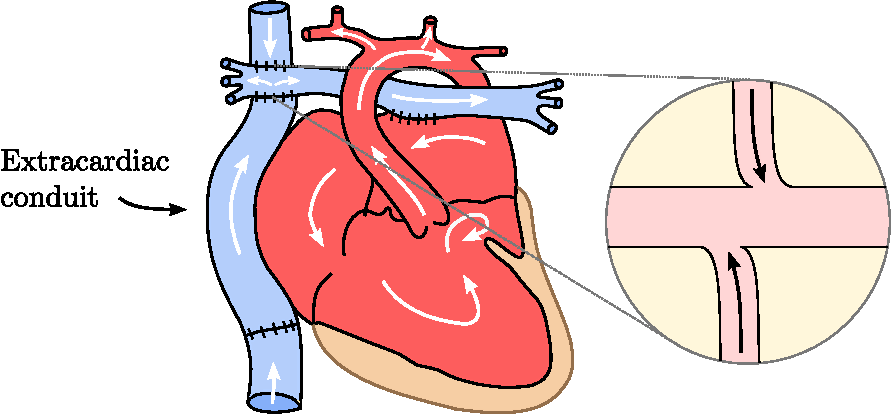
\includegraphics[width=0.9\linewidth]{Images/srdce_zoom.pdf}
			\end{figure}
		\end{column}%
		\hfill%
		\begin{column}{.37\textwidth}
			\vspace{0pt}
			\textbf{Optimization problem:}\\
			\vspace{6pt}
			Finding the minimum value
			\begin{equation*}
				\min _{\vect{x} \in \mathbb{X} } f \ (\vect{x}),
			\end{equation*}
			$ f \ (\vect{x}) $ is the objective function.\\ \pause
			\vspace{11pt}
			\textbf{Characteristics:}\\[2pt]
			\begin{itemize}
				\item non-linear
				\item constrained
			\end{itemize}
		\end{column}%
	\end{columns}
\end{frame}

%------------------------------------------------
\section{Pipeline}
%------------------------------------------------
\begin{frame}{Pipeline}
	
	\begin{figure}
		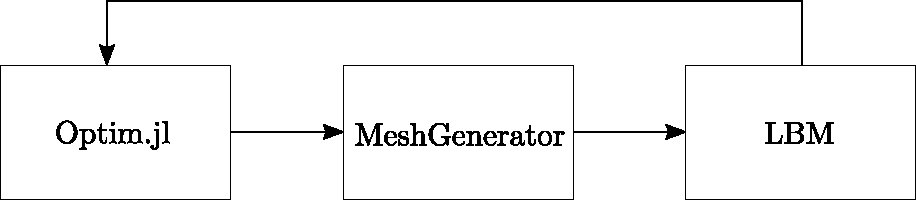
\includegraphics[width=0.9\linewidth, trim={0 -0.1cm 0 0}, clip]{Images/pipeline.pdf}
	\end{figure}
	\vspace{-2mm}
	\begin{columns}[T] % align columns
		\begin{column}{.31\textwidth}
			\begin{figure}
				
\includegraphics[width=0.5\linewidth, trim={0 0 0 0}, clip]{Images/julia.png}
			\end{figure}
		\end{column}%
		\begin{column}{.31\textwidth}
			\begin{figure}
				
\includegraphics[width=0.35\linewidth, trim={0 0 0 0cm}, clip]{Images/python.png}
			\end{figure}
		\end{column}%
		\begin{column}{.31\textwidth}
			\begin{figure}
				
\includegraphics[width=0.35\linewidth, trim={0 0 0 0cm}, clip]{Images/cpp.png}
			\end{figure}
		\end{column}%	
	\end{columns}
\end{frame}
%------------------------------------------------
\begin{frame}{Pipeline}
	\addtocounter{framenumber}{-1}
	\begin{figure}
		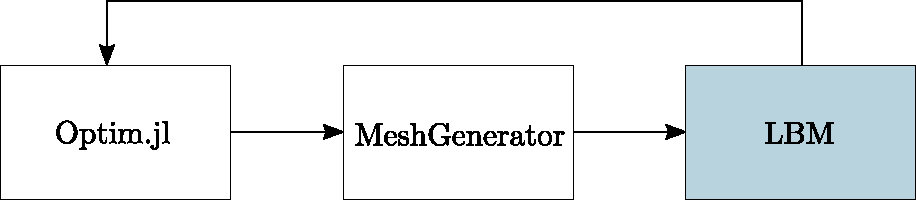
\includegraphics[width=0.9\linewidth, trim={0 -0.1cm 0 0}, clip]{Images/pipeline3.pdf}
	\end{figure}
	\vspace{-2mm}
	\begin{columns}[T] % align columns
		\begin{column}{.31\textwidth}
			\begin{figure}
				
\includegraphics[width=0.5\linewidth, trim={0 0 0 0}, clip]{Images/julia.png}
			\end{figure}
		\end{column}%
		\begin{column}{.31\textwidth}
			\begin{figure}
				
\includegraphics[width=0.35\linewidth, trim={0 0 0 0cm}, clip]{Images/python.png}
			\end{figure}
		\end{column}%
		\begin{column}{.31\textwidth}
			\begin{figure}
				
\includegraphics[width=0.35\linewidth, trim={0 0 0 0cm}, clip]{Images/cpp.png}
			\end{figure}
		\end{column}%	
	\end{columns}
\end{frame}
%------------------------------------------------
\begin{frame}{Lattice Boltzmann method}
	\begin{columns}[T] % align columns
		\begin{column}{.45\textwidth}
			\textbf{LBM:}\\
			\begin{itemize}
				\item velocity set D2Q9, CLBM
				\item in-house implementation
			\end{itemize}
		\begin{eqnarray*}
			\rho &=& \sum_{k=0}^{q-1} f_{k}\\[3pt]
			\rho \vect{u} &=& \sum_{k=0}^{q-1} f_{k} \boldsymbol{\xi}_{k} + \dfrac{\Delta t}{2} \rho \boldsymbol{g}
		\end{eqnarray*}
		\end{column}%
		\begin{column}{.5\textwidth}
			\textbf{Fluid dynamics equations:}
			\vspace{-13pt}
			\begin{center}
				$$\frac{\partial \rho}{\partial t} + \nabla \cdot (\rho \vect{u}) = 0 $$
				$$\frac{\partial (\rho \vect{u})}{\partial t} + \nabla \cdot (\rho \vect{u} \otimes \vect{u}) = \nabla \cdot \mathbf{T} + \rho \boldsymbol{g}$$
			\end{center}%
			\vspace{11pt}
			\textbf{Assumptions:}\\[2pt]
			\begin{itemize}
				\item isothermal system, no external forces
				\item incompressible Newtonian fluid
			\end{itemize}
		\end{column}%
	\end{columns}
\end{frame}
%------------------------------------------------
\begin{frame}{LBM - boundary conditions}
	\begin{columns}[T] % align columns
		\begin{column}{.55\textwidth}
			\begin{itemize}
				\item domain boundary $ \rightarrow $ moment-based BC [1]
				\begin{itemize}
					\vspace{-3mm}
					\item unknown DDFs from the known DDFs and known macroscopic moments
					\vspace{1mm}
				\end{itemize}
				\item object boundary $ \rightarrow $ interpolation BC [2]
				\begin{itemize}
					\vspace{1mm}
					\item better representation of curved boundary
					\vspace{1mm}
				\end{itemize}
			\end{itemize}
		\end{column}%
		\begin{column}{.45\textwidth}
			\begin{figure}
				\vspace{-0.5cm}
				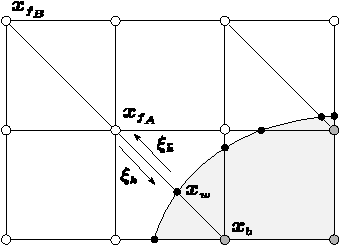
\includegraphics[width=0.78\linewidth, trim={0 0 0 0}, clip]{Images/bouzidi.pdf}
			\end{figure}
		\end{column}%
	\end{columns}
	\vspace{4.5mm}
	\begin{columns}
		\begin{column}{.63\textwidth}
			$\begin{aligned}
				& \Theta<\frac{1}{2}: \ \ f_{\bar{k}}\left(\boldsymbol{x}_{f_A}, t+\Delta t\right)=2 \Theta f_k^*\left(\boldsymbol{x}_{f_A}, t\right)+(1-2 \Theta) f_k^*\left(\boldsymbol{x}_{f_B}, t\right) \\
				& \Theta \geq \frac{1}{2}: \ \ f_{\bar{k}}\left(\boldsymbol{x}_{f_A}, t+\Delta t\right)=\frac{1}{2 \Theta} f_k^*\left(\boldsymbol{x}_{f_A}, t\right)+\frac{2 \Theta-1}{2 \Theta} f_{\bar{k}}^*\left(\boldsymbol{x}_{f_A}, t\right)
			\end{aligned}$
		\end{column}
		\begin{column}{.25\textwidth}
			\begin{figure}
				$ \color{teal}
				\Theta=\frac{{\parallel}\boldsymbol{x}_{f_A}-\boldsymbol{x}_w {\parallel}}{{\parallel}\boldsymbol{x}_{f_A}-\boldsymbol{x}_b{\parallel}}$
			\end{figure}
		\end{column}%
	\end{columns}
	\vspace{3.5mm}
	\tiny{[1] Eichler P. (2023)}, \textit{Mathematical modeling of fluid flow using lattice Boltzmann
		method.}, Dissertation\\
	\tiny{[2] Bouzidi M., et al. (2001), \textit{Momentum transfer of a Boltzmann-lattice fluid with boundaries},  doi: 10.1063/1.1399290}

\end{frame}
%------------------------------------------------
\begin{frame}{Pipeline}
	\addtocounter{framenumber}{-1}
	\begin{figure}
		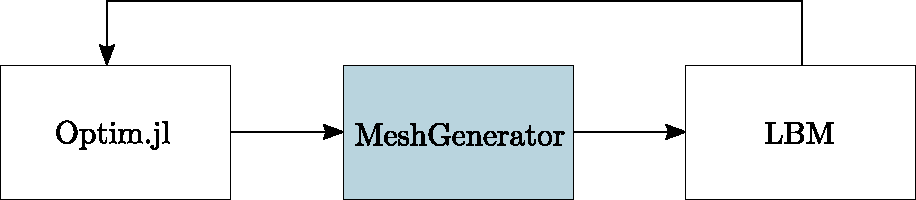
\includegraphics[width=0.9\linewidth, trim={0 -0.1cm 0 0}, clip]{Images/pipeline2.pdf}
	\end{figure}
	\vspace{-2mm}
	\begin{columns}[T] % align columns
		\begin{column}{.31\textwidth}
			\begin{figure}
				
\includegraphics[width=0.5\linewidth, trim={0 0 0 0}, clip]{Images/julia.png}
			\end{figure}
		\end{column}%
		\begin{column}{.31\textwidth}
			\begin{figure}
				
\includegraphics[width=0.35\linewidth, trim={0 0 0 0cm}, clip]{Images/python.png}
			\end{figure}
		\end{column}%
		\begin{column}{.31\textwidth}
			\begin{figure}
				
\includegraphics[width=0.35\linewidth, trim={0 0 0 0cm}, clip]{Images/cpp.png}
			\end{figure}
		\end{column}%	
	\end{columns}
\end{frame}
%------------------------------------------------
\begin{frame}{Generating the geometry}
	\begin{columns}
		\begin{column}{.52\textwidth}
			\begin{itemize}
				\setlength\itemsep{2em}
				\uncover<1->{
				\item Package \texttt{meshgenerator} implemented in Python
				\item Rigid object $ \Rightarrow $ precalculate known values 
				\item Various possible objects - parametrization}
%			\uncover<2->{
%				\item \alert{Sidequest} - real-life experiments using MRI $ \Rightarrow $ 3D printing
%				\vspace{0.5cm}
%			
%				\begin{figure}
%					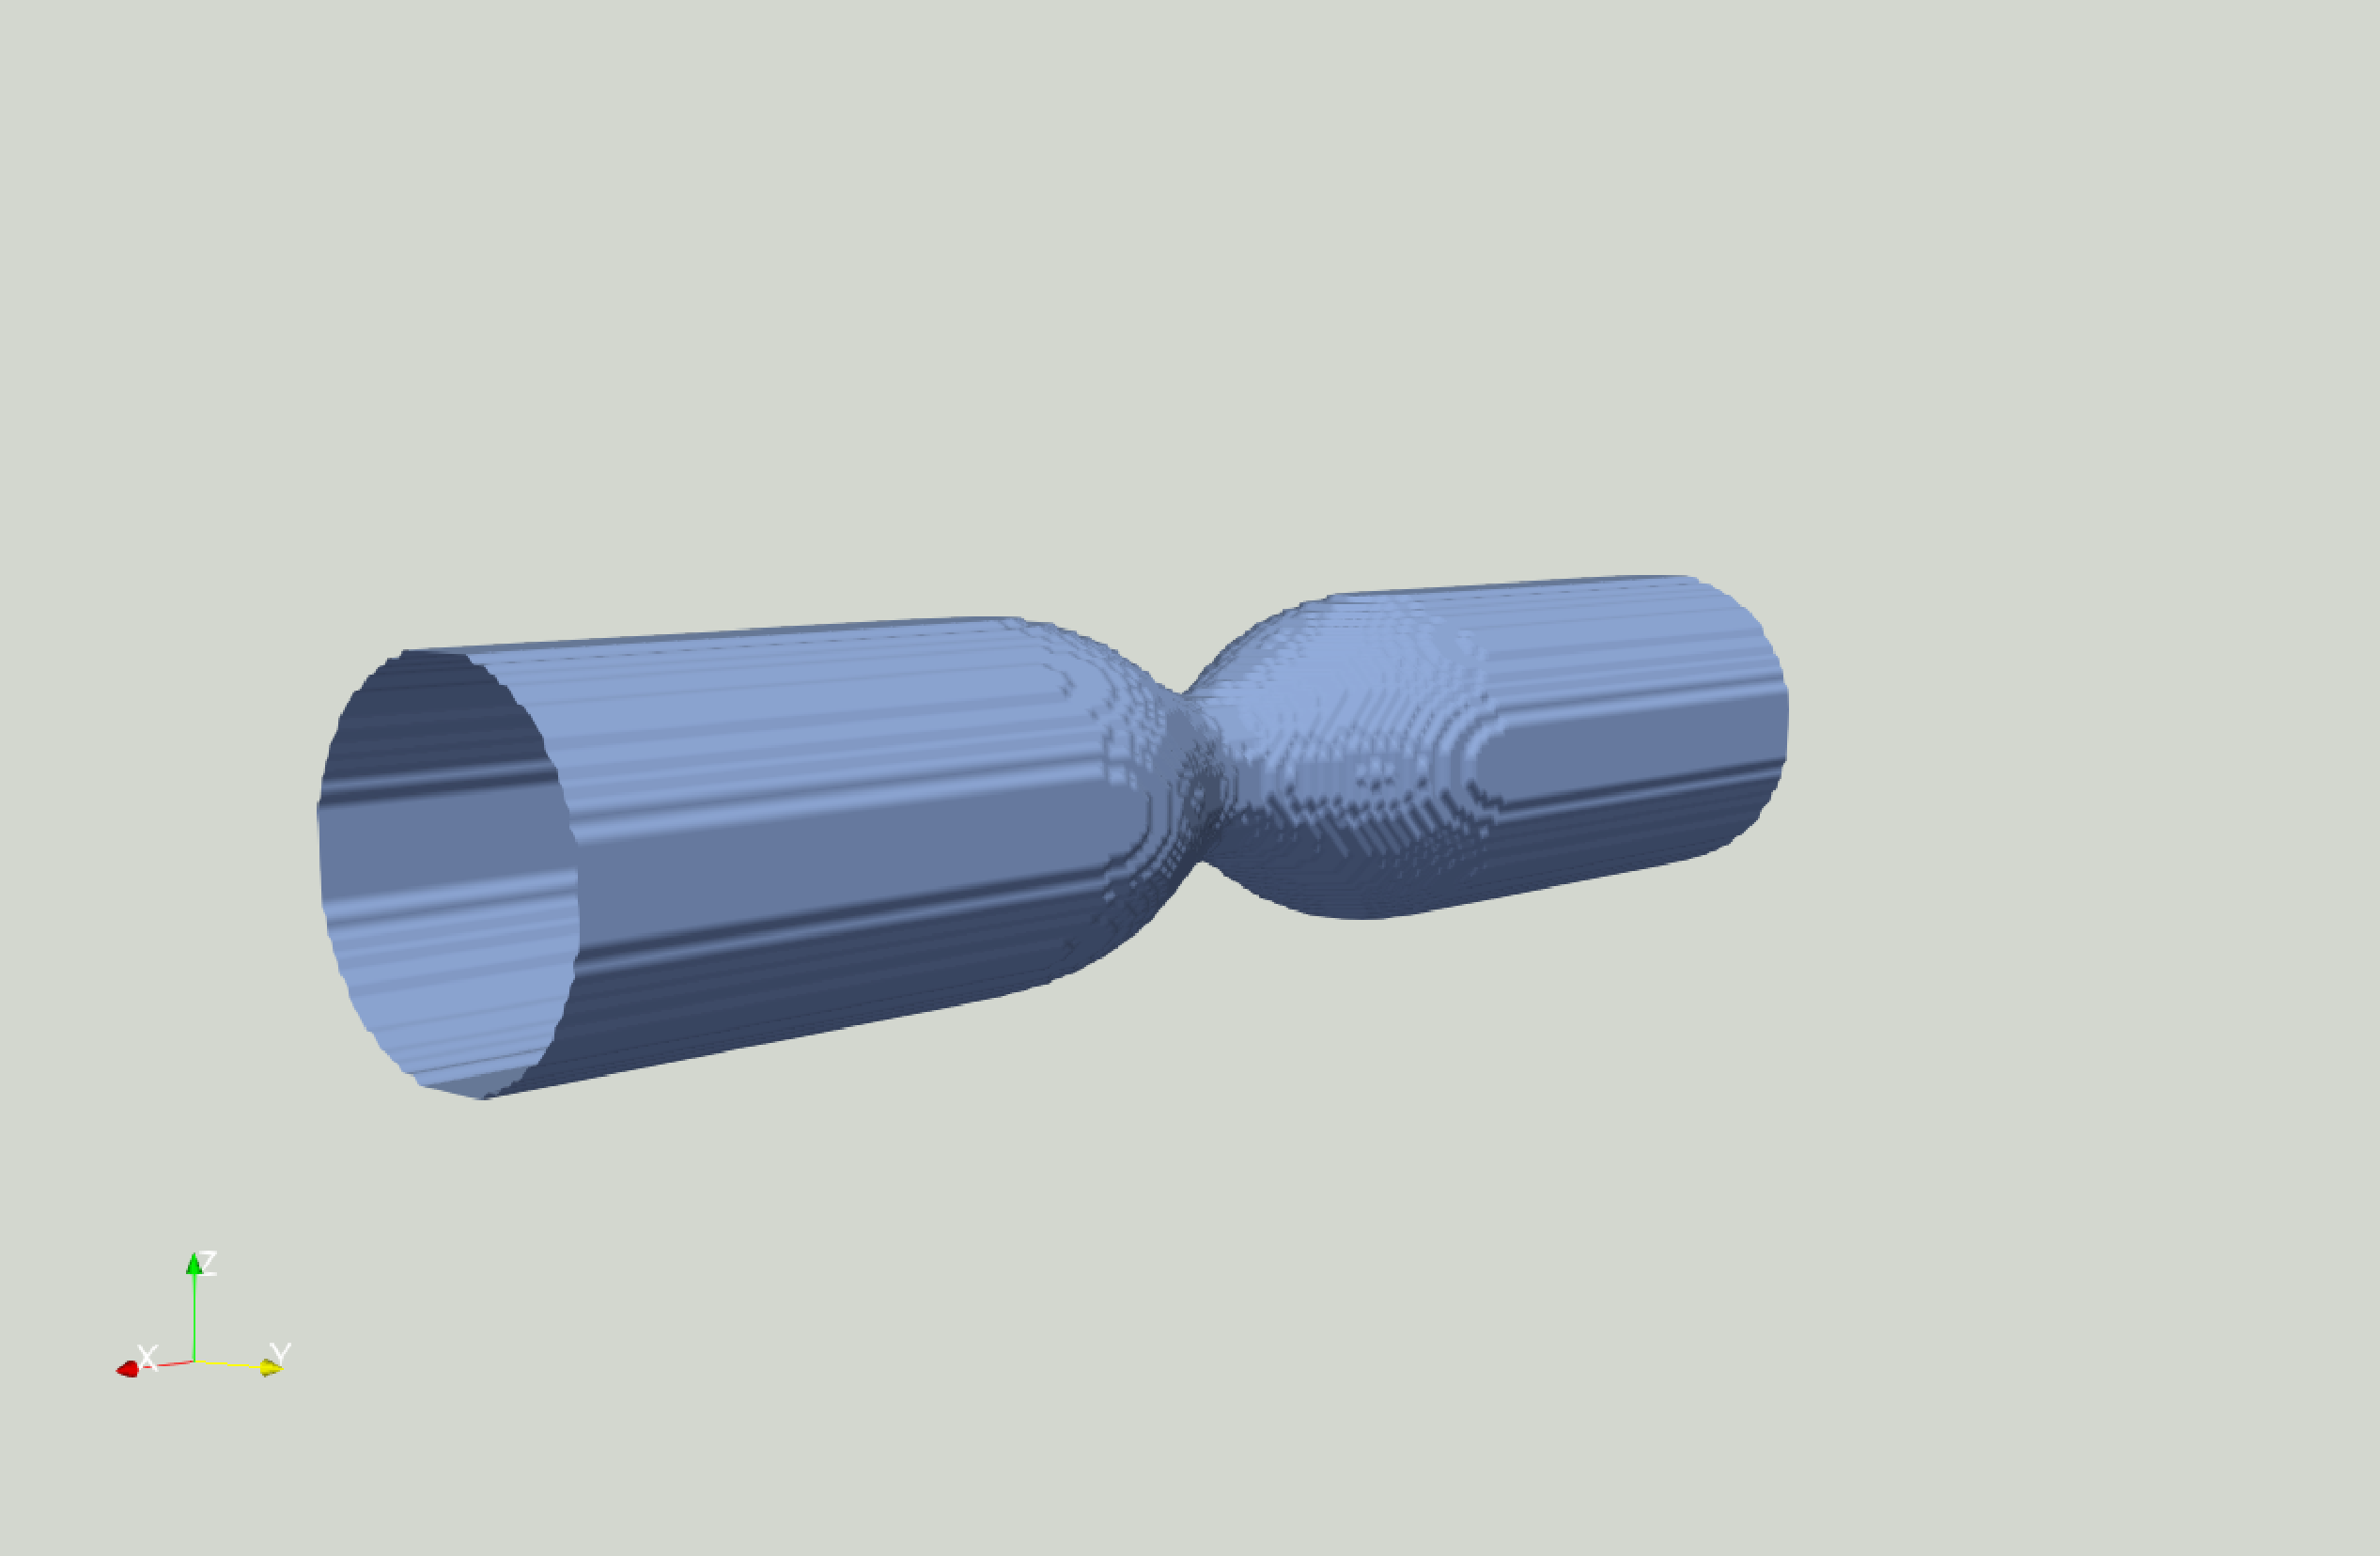
\includegraphics[width=0.75\linewidth, trim={3.0cm 5.5cm 8.5cm 7.5cm}, clip]{Images/vessel.pdf}
%				\end{figure}
%			}
			\end{itemize}
		\end{column}
		\uncover<1->{
		\begin{column}[c]{.47\textwidth}
			\begin{figure}
				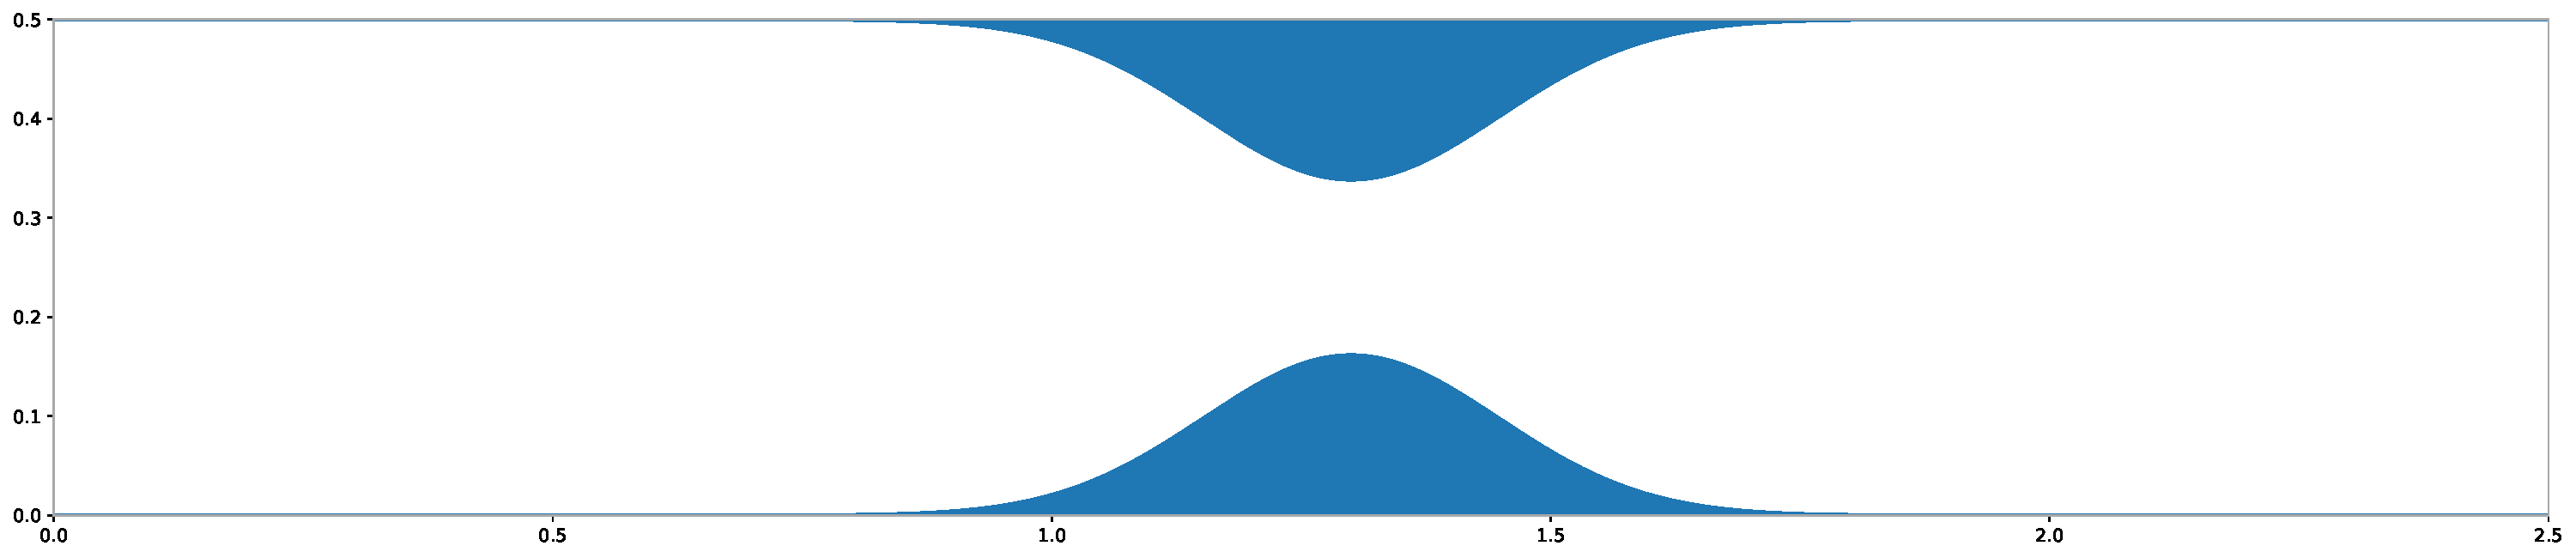
\includegraphics[width=0.9\linewidth, trim={0 0 0 0cm}, clip]{Images/figvessel.pdf}
			\end{figure}
			\begin{figure}
			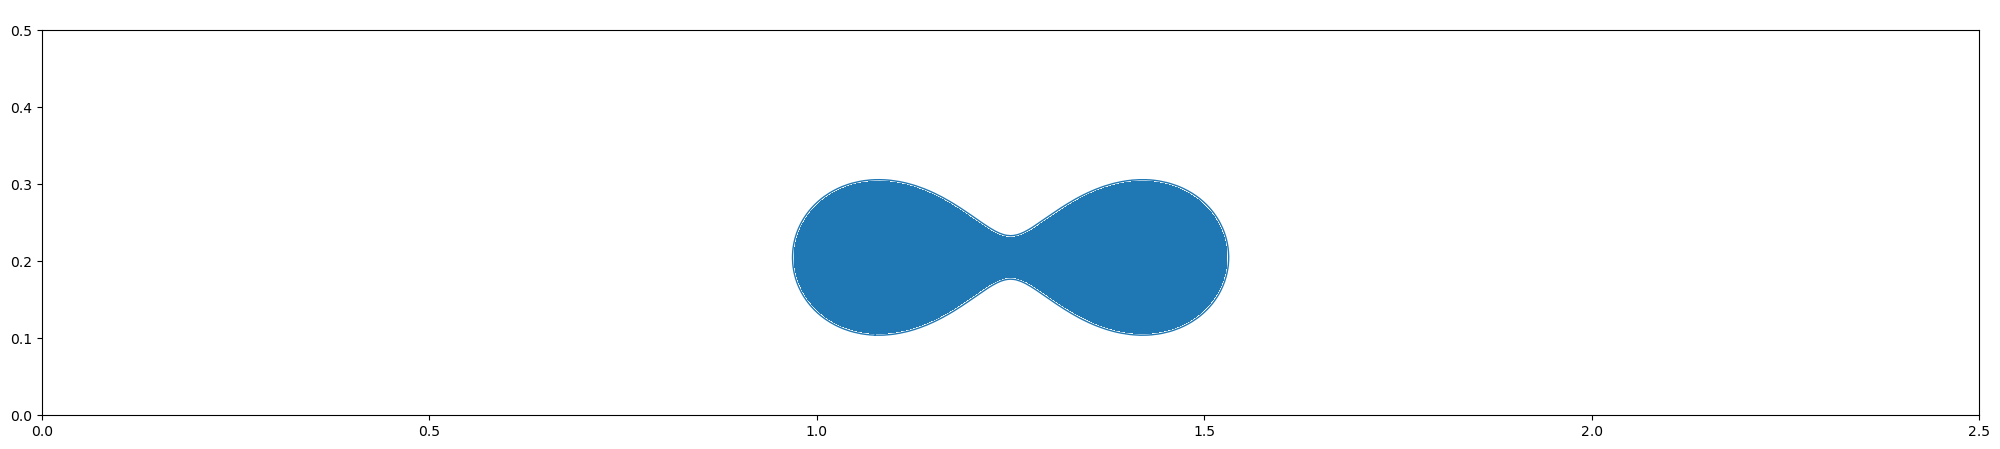
\includegraphics[width=0.9\linewidth, trim={0 0 0 0cm}, clip]{Images/c1.png}
			\end{figure}
			\begin{figure}
			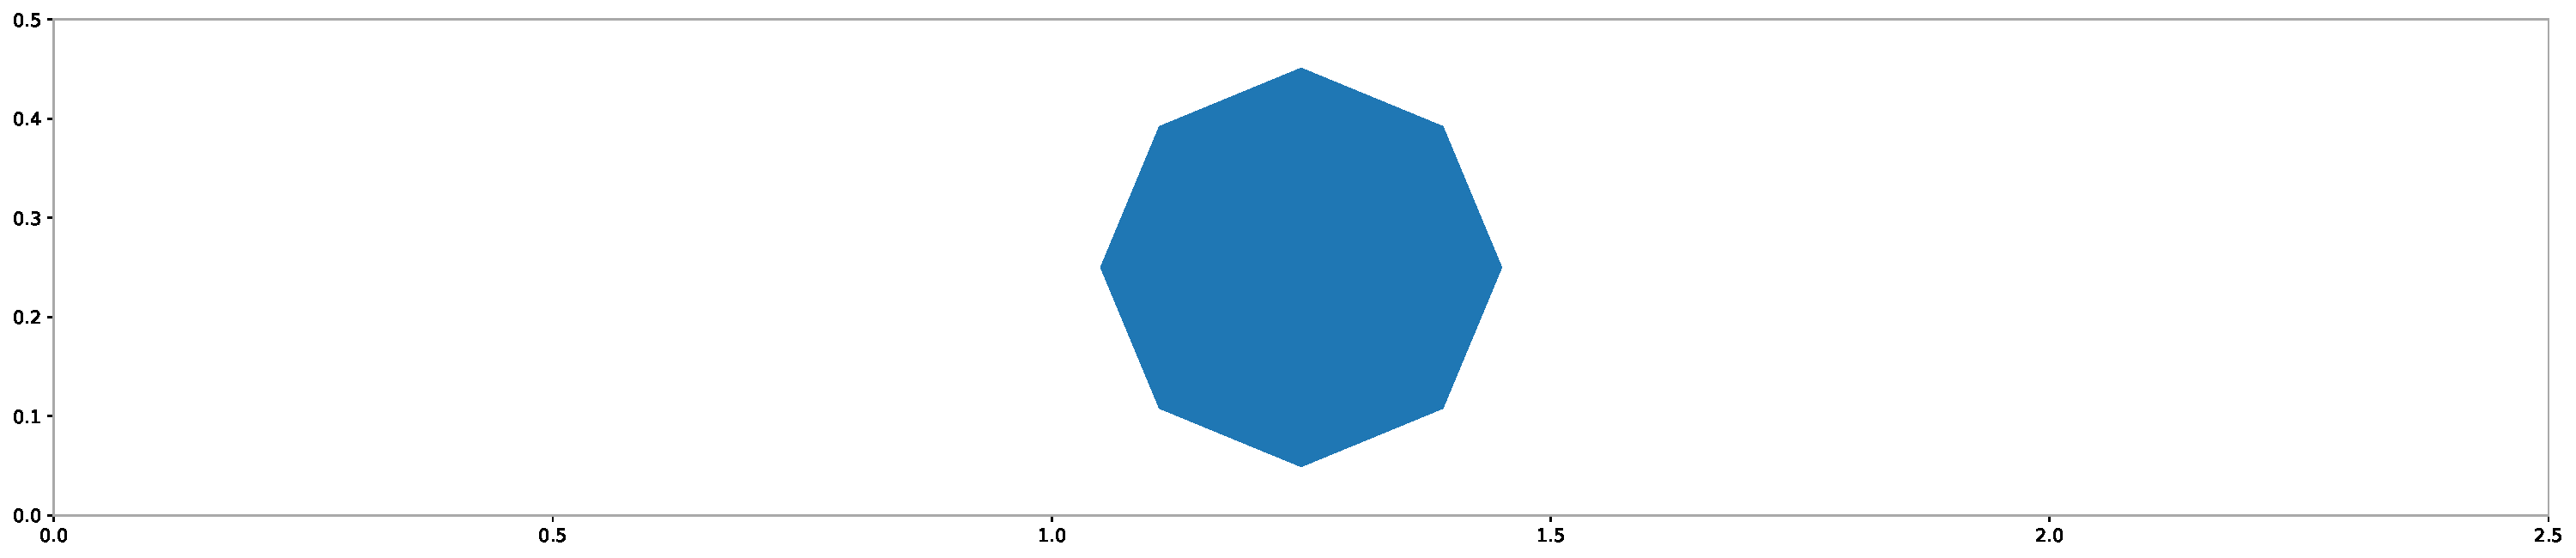
\includegraphics[width=0.9\linewidth, trim={0 0 0 0cm}, clip]{Images/figoktagon.pdf}
			\end{figure}
		\end{column}
	}
	
	\end{columns}

\end{frame}
%------------------------------------------------
\begin{frame}{Pipeline}
	\addtocounter{framenumber}{-1}
	\begin{figure}
		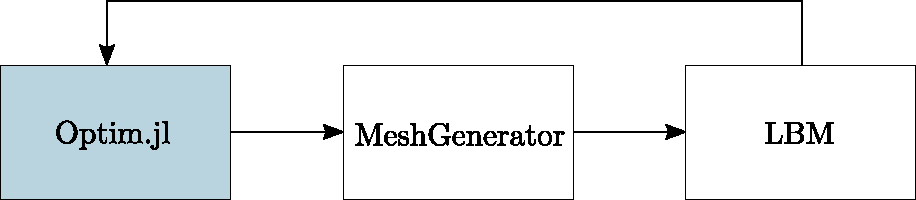
\includegraphics[width=0.9\linewidth, trim={0 -0.1cm 0 0}, clip]{Images/pipeline1.pdf}
	\end{figure}
	\vspace{-2mm}
	\begin{columns}[T] % align columns
		\begin{column}{.31\textwidth}
			\begin{figure}
				
\includegraphics[width=0.5\linewidth, trim={0 0 0 0}, clip]{Images/julia.png}
			\end{figure}
		\end{column}%
		\begin{column}{.31\textwidth}
			\begin{figure}
				
\includegraphics[width=0.35\linewidth, trim={0 0 0 0cm}, clip]{Images/python.png}
			\end{figure}
		\end{column}%
		\begin{column}{.31\textwidth}
			\begin{figure}
				
\includegraphics[width=0.35\linewidth, trim={0 0 0 0cm}, clip]{Images/cpp.png}
			\end{figure}
		\end{column}%	
	\end{columns}
\end{frame}
%------------------------------------------------
\begin{frame}{Optimisation}
	\begin{itemize}
		\setlength\itemsep{1.4em}
		\item \texttt{Optim} - Julia package
		\item Constrained problem $\Rightarrow$ extreme barrier method
		\item Algorithms: L-BFGS, Nelder-Mead (gradient free)
		\item Evaluating $ f \ (x) $ using LBM $\Rightarrow$ \alert{expensive}
		\item Evaluating $ \nabla f \ (x) $ using LBM $\Rightarrow$ \alert{even more expensive}
	\end{itemize}
\end{frame}


%------------------------------------------------
\section{Results}
%------------------------------------------------
\begin{frame}{Results}
	\begin{itemize}
		\setlength\itemsep{1.4em}
		\item Using \texttt{MeshGenerator} package, defining non-trivial problems
		\item Reynolds' decomposition:
				$$ \vect{u} \,(x, y, z, t) = \overline{\vect{u} \,(x, y, z)} + \vect{u}^\prime(x, y, z, t) $$
		\item Objective function: Turbulence kinetic energy and shear rate
				$$ T_{\mathrm{turb}} = \frac{1}{2} (\vect{u}^\prime(x, y, z, t) )^2, \hspace{5mm} \dot{\gamma} = \sqrt{2} || \, \mathbf{D} \, ||^{}_{F}$$
		\item Incompressible Newtonian fluid, 2D
	\end{itemize}
\end{frame}

%------------------------------------------------
\begin{frame}{1 parameter - rotating ellipse}
	\begin{itemize}
		\item angle of rotation $ \theta $ is the only parameter
		\vspace{7mm}
	\end{itemize}
	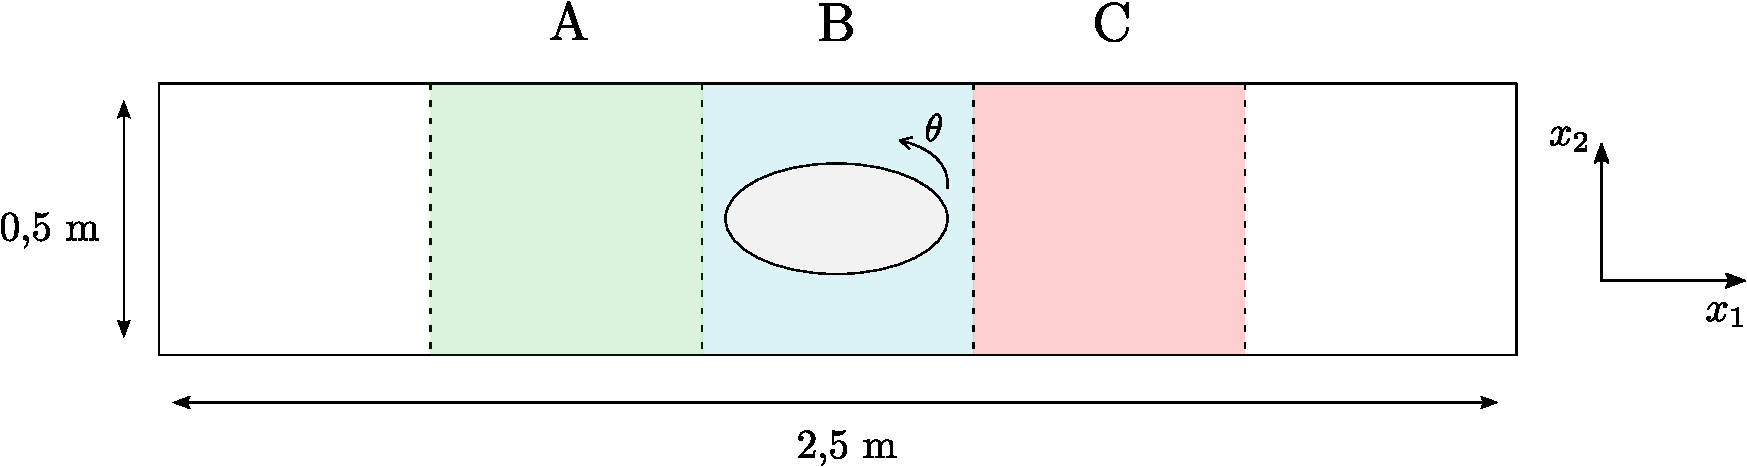
\includegraphics[width=1\linewidth, trim={0 0 0 0}, clip]{Images/elipsa1.pdf}	
\end{frame}
%------------------------------------------------
\begin{frame}{1 parameter - rotating ellipse}
	\addtocounter{framenumber}{-1}
	\begin{columns}
		\begin{column}{.56\textwidth}
			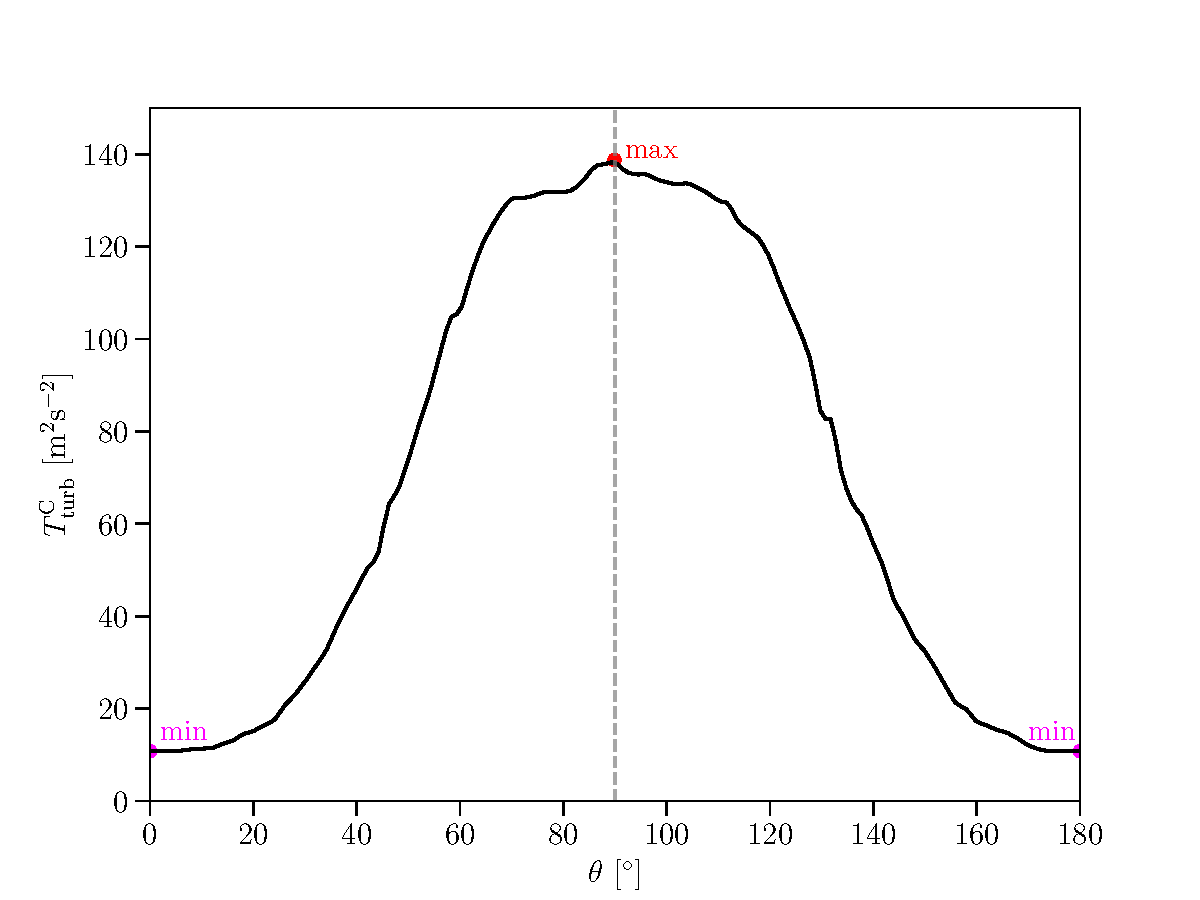
\includegraphics[width=1\linewidth, trim={0 0 0 0}, clip]{Images/elip1interpolated.pdf}			
		\end{column}
		\begin{column}{.52\textwidth}
			Minimum:\\[4pt]
			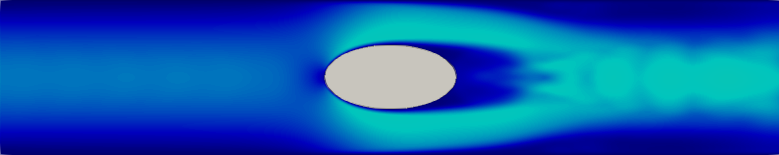
\includegraphics[width=0.9\linewidth, trim={0 0 0 0}, clip]{Images/ellipse1_min_a.png}
			\\ \vspace{2mm}
			Maximum:\\[4pt]	
			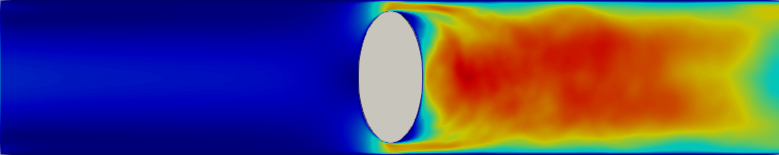
\includegraphics[width=0.9\linewidth, trim={0 0 0 0}, clip]{Images/ellipse1_max_a.png}
			\\ \vspace{4mm}		
			\centering
			\hspace{-6mm}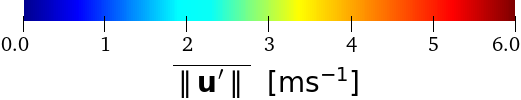
\includegraphics[width=0.6\linewidth, trim={0 0 0 0}, clip]{Images/ellipse12_legenda.png}
		\end{column}
	\end{columns}
\end{frame}
%------------------------------------------------
\begin{frame}{1 parameter - rotating ellipse}
	\begin{itemize}
		\item angle of rotation $ \theta $ is the only parameter
		\vspace{7mm}
	\end{itemize}
	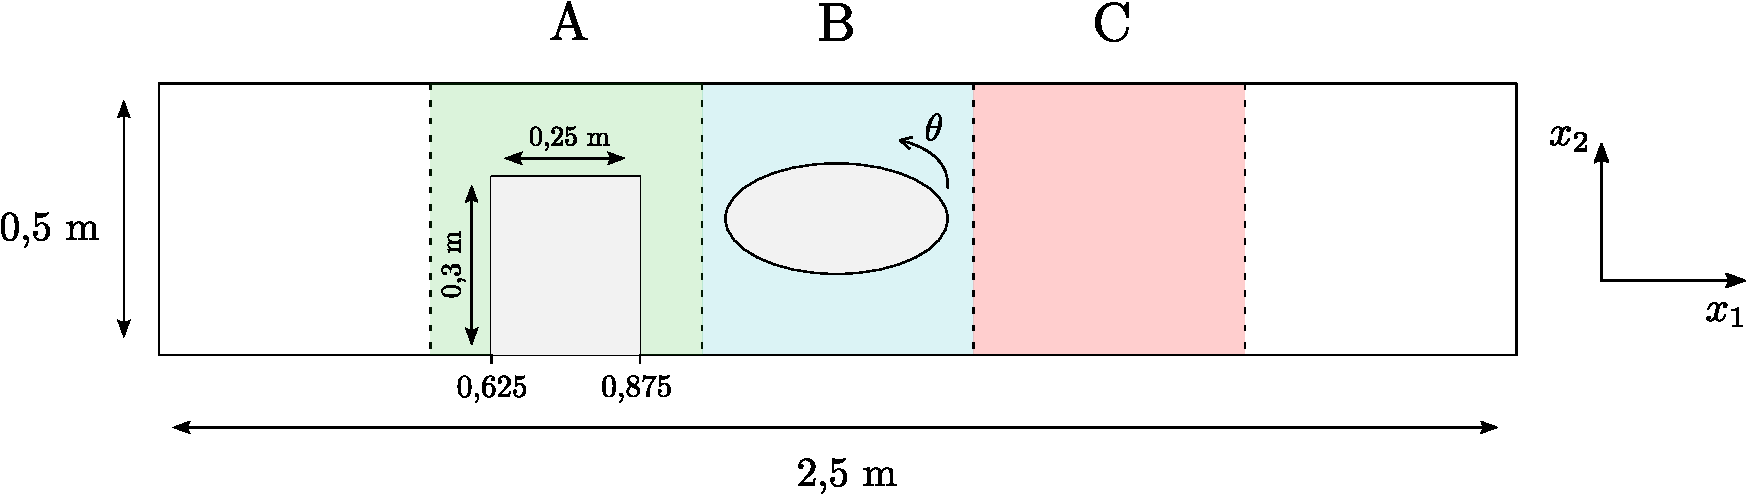
\includegraphics[width=1\linewidth, trim={0 0 0 0}, clip]{Images/elipsa2.pdf}			
\end{frame}
%------------------------------------------------
\begin{frame}{1 parameter - rotating ellipse}
	\addtocounter{framenumber}{-1}
	\begin{columns}
		\begin{column}{.56\textwidth}
			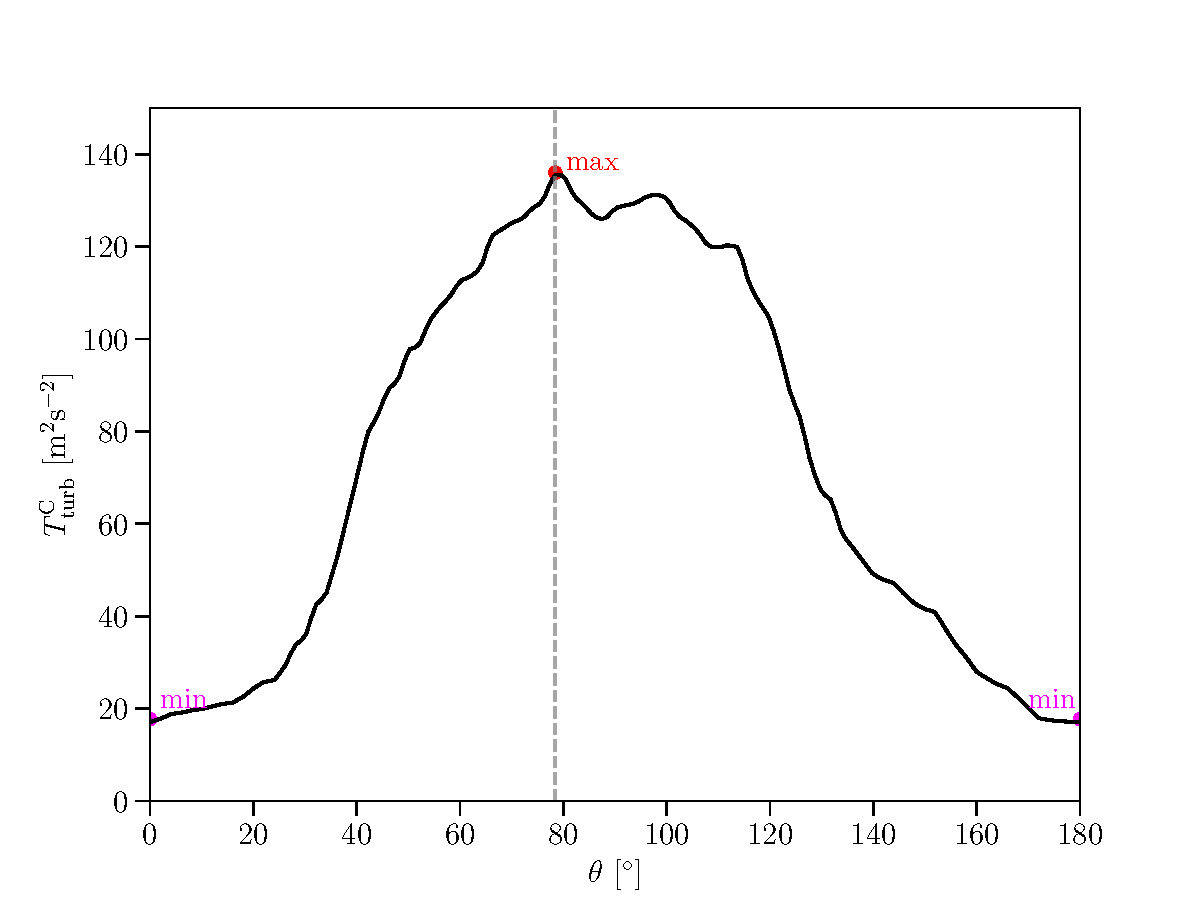
\includegraphics[width=1\linewidth, trim={0 0 0 0}, clip]{Images/elip2interpolated.pdf}			
		\end{column}
		\begin{column}{.52\textwidth}
			Minimum:\\[4pt]
			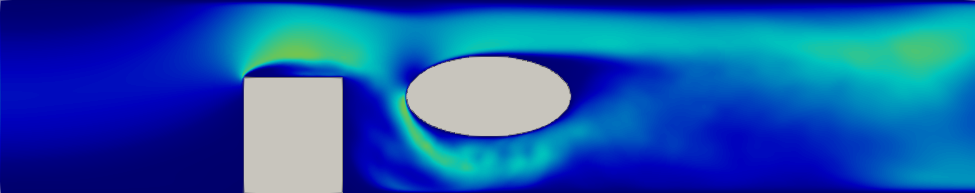
\includegraphics[width=0.9\linewidth, trim={0 0 0 0}, clip]{Images/ellipse2_min_aa.png}
			\\ \vspace{2mm}
			Maximum:\\[4pt]	
			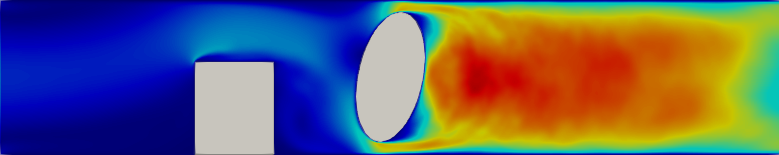
\includegraphics[width=0.9\linewidth, trim={0 0 0 0}, clip]{Images/ellipse2_max_a.png}
			\\ \vspace{4mm}		
			\centering
			\hspace{-6mm}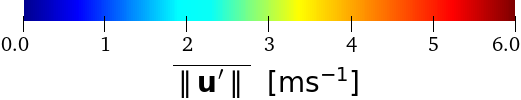
\includegraphics[width=0.6\linewidth, trim={0 0 0 0}, clip]{Images/ellipse12_legenda.png}
		\end{column}
	\end{columns}
\end{frame}
%------------------------------------------------
\begin{frame}{2 parameters - changing Cassinian oval}
	\begin{columns}
		\begin{column}{.6\textwidth}
			\begin{itemize}
				\setlength\itemsep{1.4em}
				\item shrinking, rotating
				\item constant area
				\item implicit equation:
			\end{itemize}		
			\vspace{4mm}
			$$ \ \ \ \ \ \ \ \ \left( x^{2}+ y^{2}+a^{2} \right)^{2}-4 x ^{2} a^{2}-b^{4} = 0 $$
			\vspace{-3mm}
			\begin{itemize}
				\item $ a $ and $ \theta $ (angle of rotation) are the parameters
			\end{itemize}	
		\end{column}
		\begin{column}{.4\textwidth}
			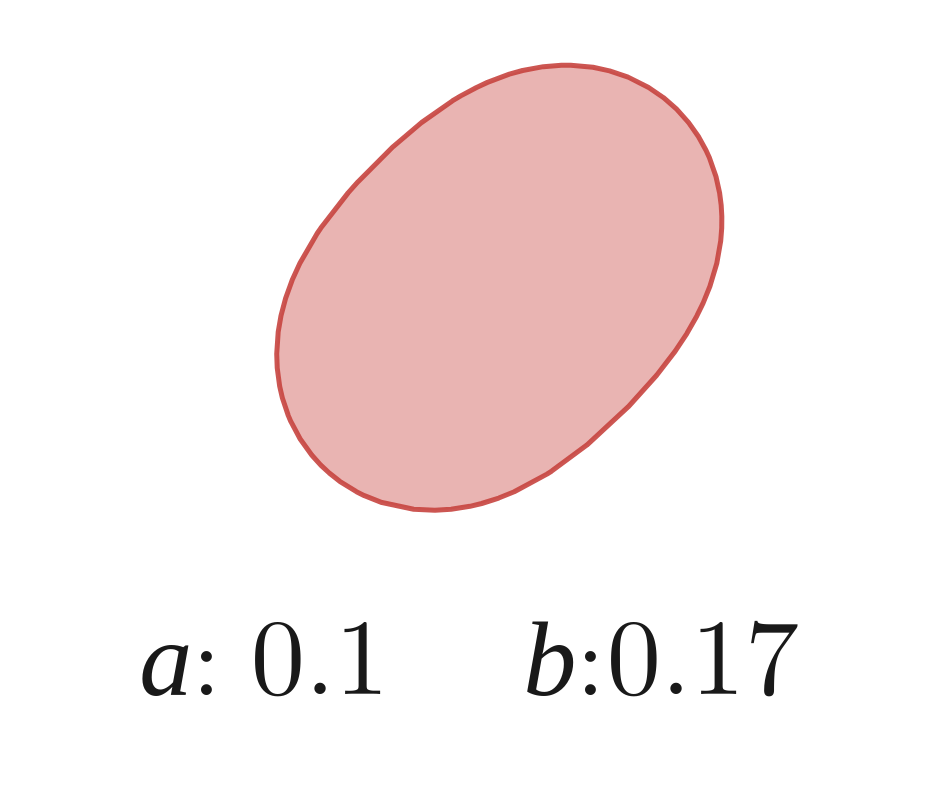
\includegraphics[width=0.9\linewidth, trim={0 0 0 0}, clip]{Images/a1.png}			
		\end{column}
	\end{columns}	
\end{frame}
%------------------------------------------------
\begin{frame}{2 parameters - changing Cassinian oval}
	\begin{columns}
		\begin{column}{.6\textwidth}
			\begin{itemize}
				\setlength\itemsep{1.4em}
				\item shrinking, rotating
				\item constant area
				\item implicit equation:
			\end{itemize}		
			\vspace{4mm}
			$$ \ \ \ \ \ \ \ \ \left( x^{2}+ y^{2}+a^{2} \right)^{2}-4 x ^{2} a^{2}-b^{4} = 0 $$
			\vspace{-3mm}
			\begin{itemize}
				\item $ a $ and $ \theta $ (angle of rotation) are the parameters
			\end{itemize}	
		\end{column}
		\begin{column}{.4\textwidth}
			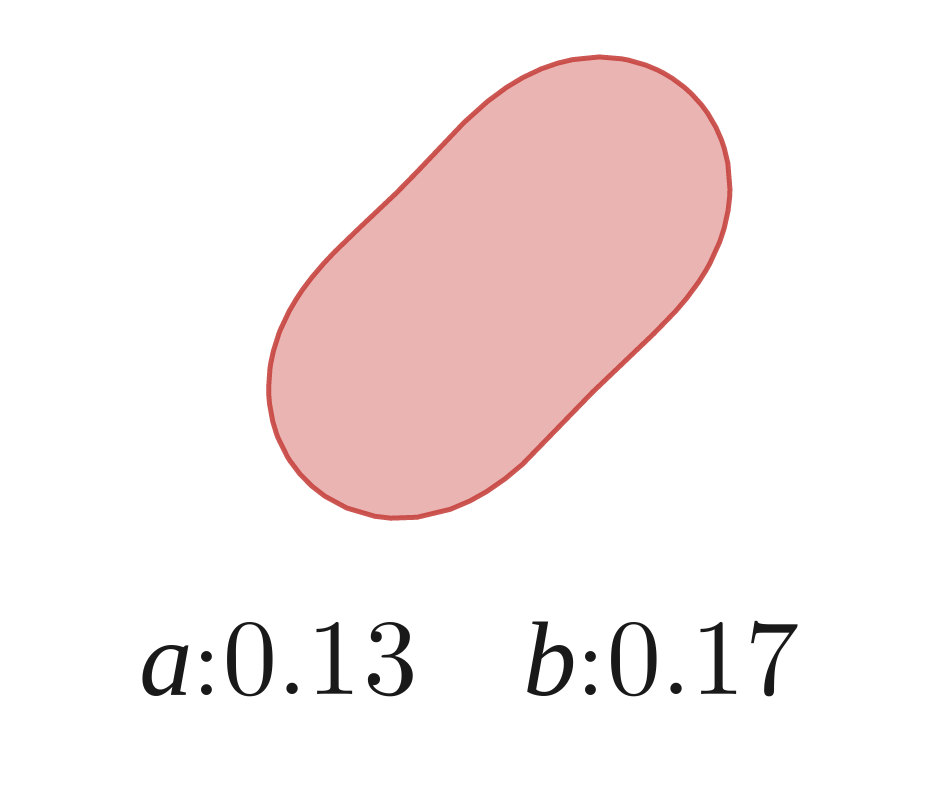
\includegraphics[width=0.9\linewidth, trim={0 0 0 0}, clip]{Images/a2.png}			
		\end{column}
	\end{columns}	
\end{frame}
%------------------------------------------------
\begin{frame}{2 parameters - changing Cassinian oval}
	\begin{columns}
		\begin{column}{.6\textwidth}
			\begin{itemize}
				\setlength\itemsep{1.4em}
				\item shrinking, rotating
				\item constant area
				\item implicit equation:
			\end{itemize}		
			\vspace{4mm}
			$$ \ \ \ \ \ \ \ \ \left( x^{2}+ y^{2}+a^{2} \right)^{2}-4 x ^{2} a^{2}-b^{4} = 0 $$
			\vspace{-3mm}
			\begin{itemize}
				\item $ a $ and $ \theta $ (angle of rotation) are the parameters
			\end{itemize}	
		\end{column}
		\begin{column}{.4\textwidth}
			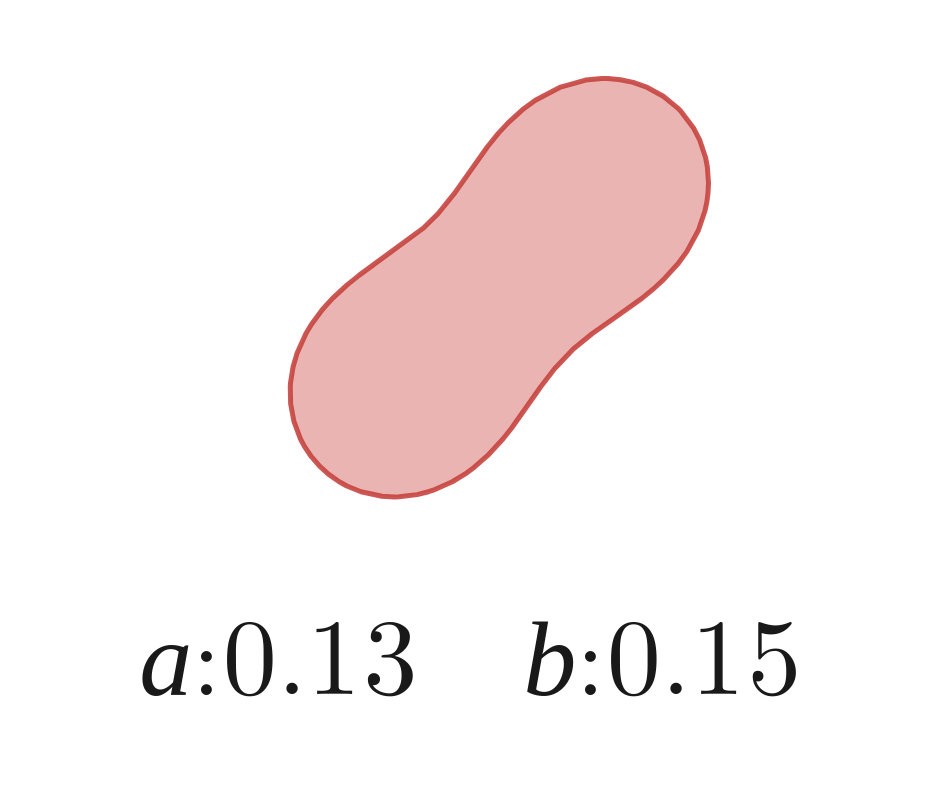
\includegraphics[width=0.9\linewidth, trim={0 0 0 0}, clip]{Images/a3.png}			
		\end{column}
	\end{columns}	
\end{frame}
%------------------------------------------------
\begin{frame}{2 parameters - changing Cassinian oval}
	\addtocounter{framenumber}{-1}
	\begin{columns}
		\begin{column}{1\textwidth}
			\begin{figure}
				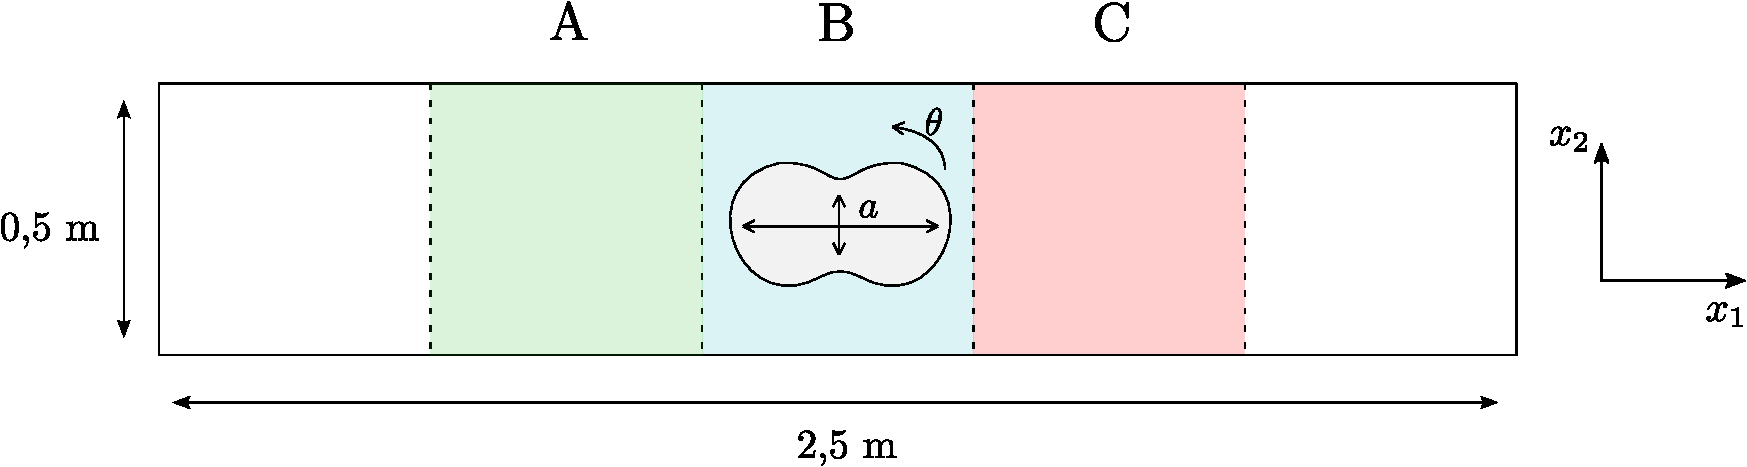
\includegraphics[width=1\linewidth, trim={0 0 0 0}, clip]{Images/cassini.pdf}		
			\end{figure}
		\end{column}
	\end{columns}	
\end{frame}
%------------------------------------------------
\begin{frame}{2 parameters - changing Cassinian oval}
	\begin{columns}
		\begin{column}{1\textwidth}
			\begin{figure}
				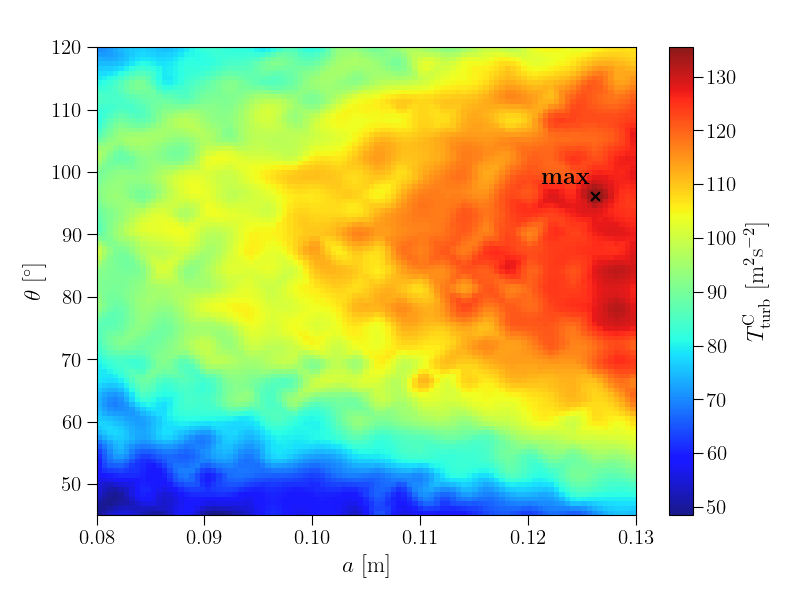
\includegraphics[width=0.68\linewidth, trim={0 0 0cm 9mm}, clip]{Images/cassini2Dinterpolated.png}		
			\end{figure}
		\end{column}
	\end{columns}	
\end{frame}

%------------------------------------------------
\begin{frame}{2 parameters - changing Cassinian oval}
	\addtocounter{framenumber}{-1}
	\begin{columns}
		\begin{column}{.55\textwidth}
			\begin{figure}
				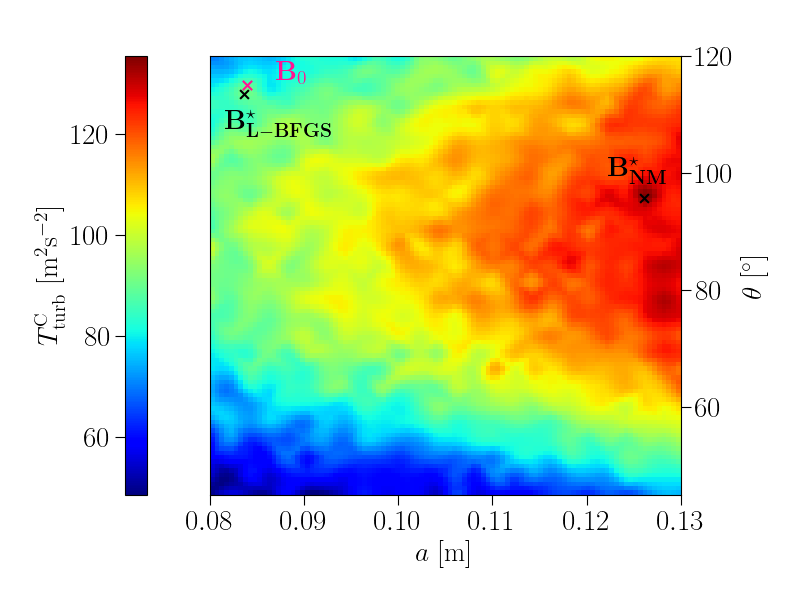
\includegraphics[width=1.1\linewidth, trim={0 0 1cm 9mm}, clip]{Images/2full.png}		
			\end{figure}
		\end{column}
		\begin{column}{.45\textwidth}
			%			\hspace{1mm}Nelder-Mead:
			\vspace{8mm}
			\begin{figure}
				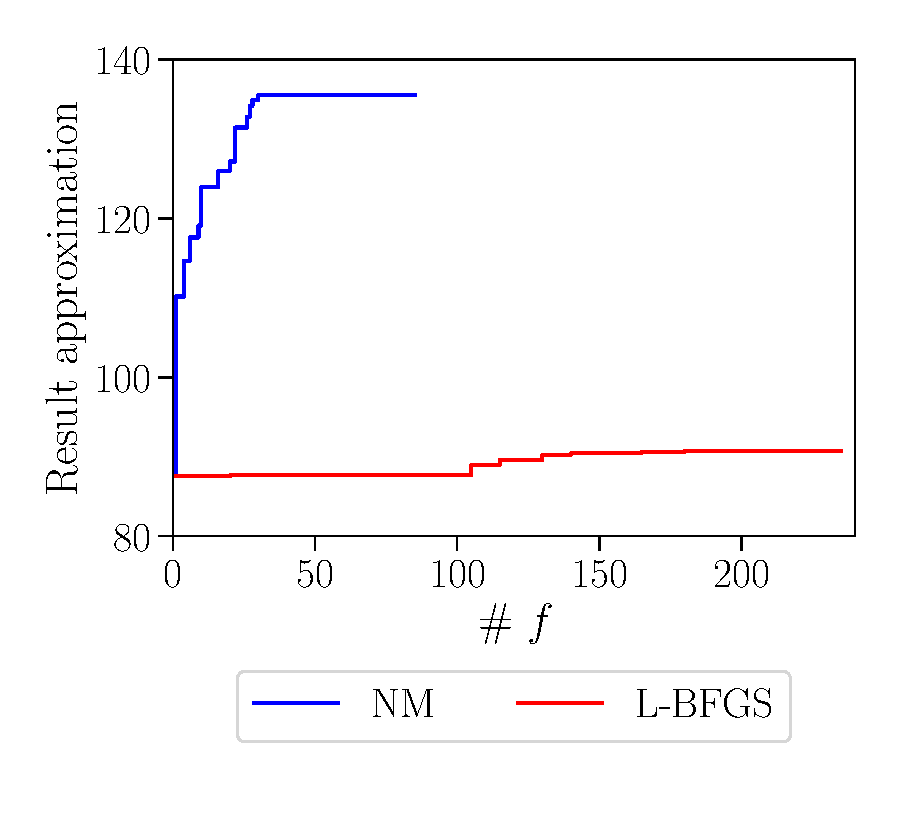
\includegraphics[width=1.0\linewidth, trim={0 0 0 9mm}, clip]{Images/7.pdf}		
			\end{figure}
			%			\vspace{0.8cm}
			%			\hspace{1mm}L-BFGS:
			%			\begin{figure}
			%				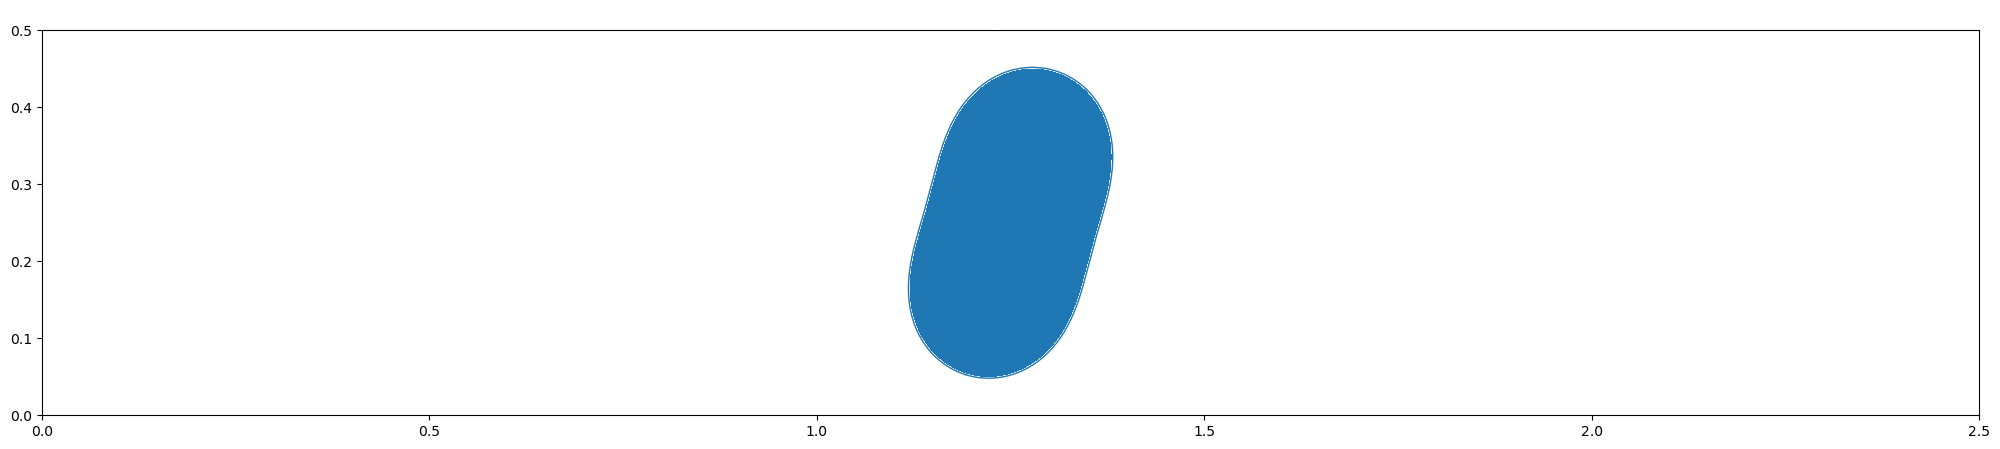
\includegraphics[width=1.0\linewidth, trim={0 0 0 9mm}, clip]{Images/bfgs.png}		
			%			\end{figure}
		\end{column}
	\end{columns}	
\end{frame}
%------------------------------------------------
\begin{frame}{3 parameters - simplified TCPC model}
	\begin{itemize}
		\item 3 optimization parameters
	\end{itemize}
	\begin{columns}
		\begin{column}{.58\textwidth}
			\begin{figure}
				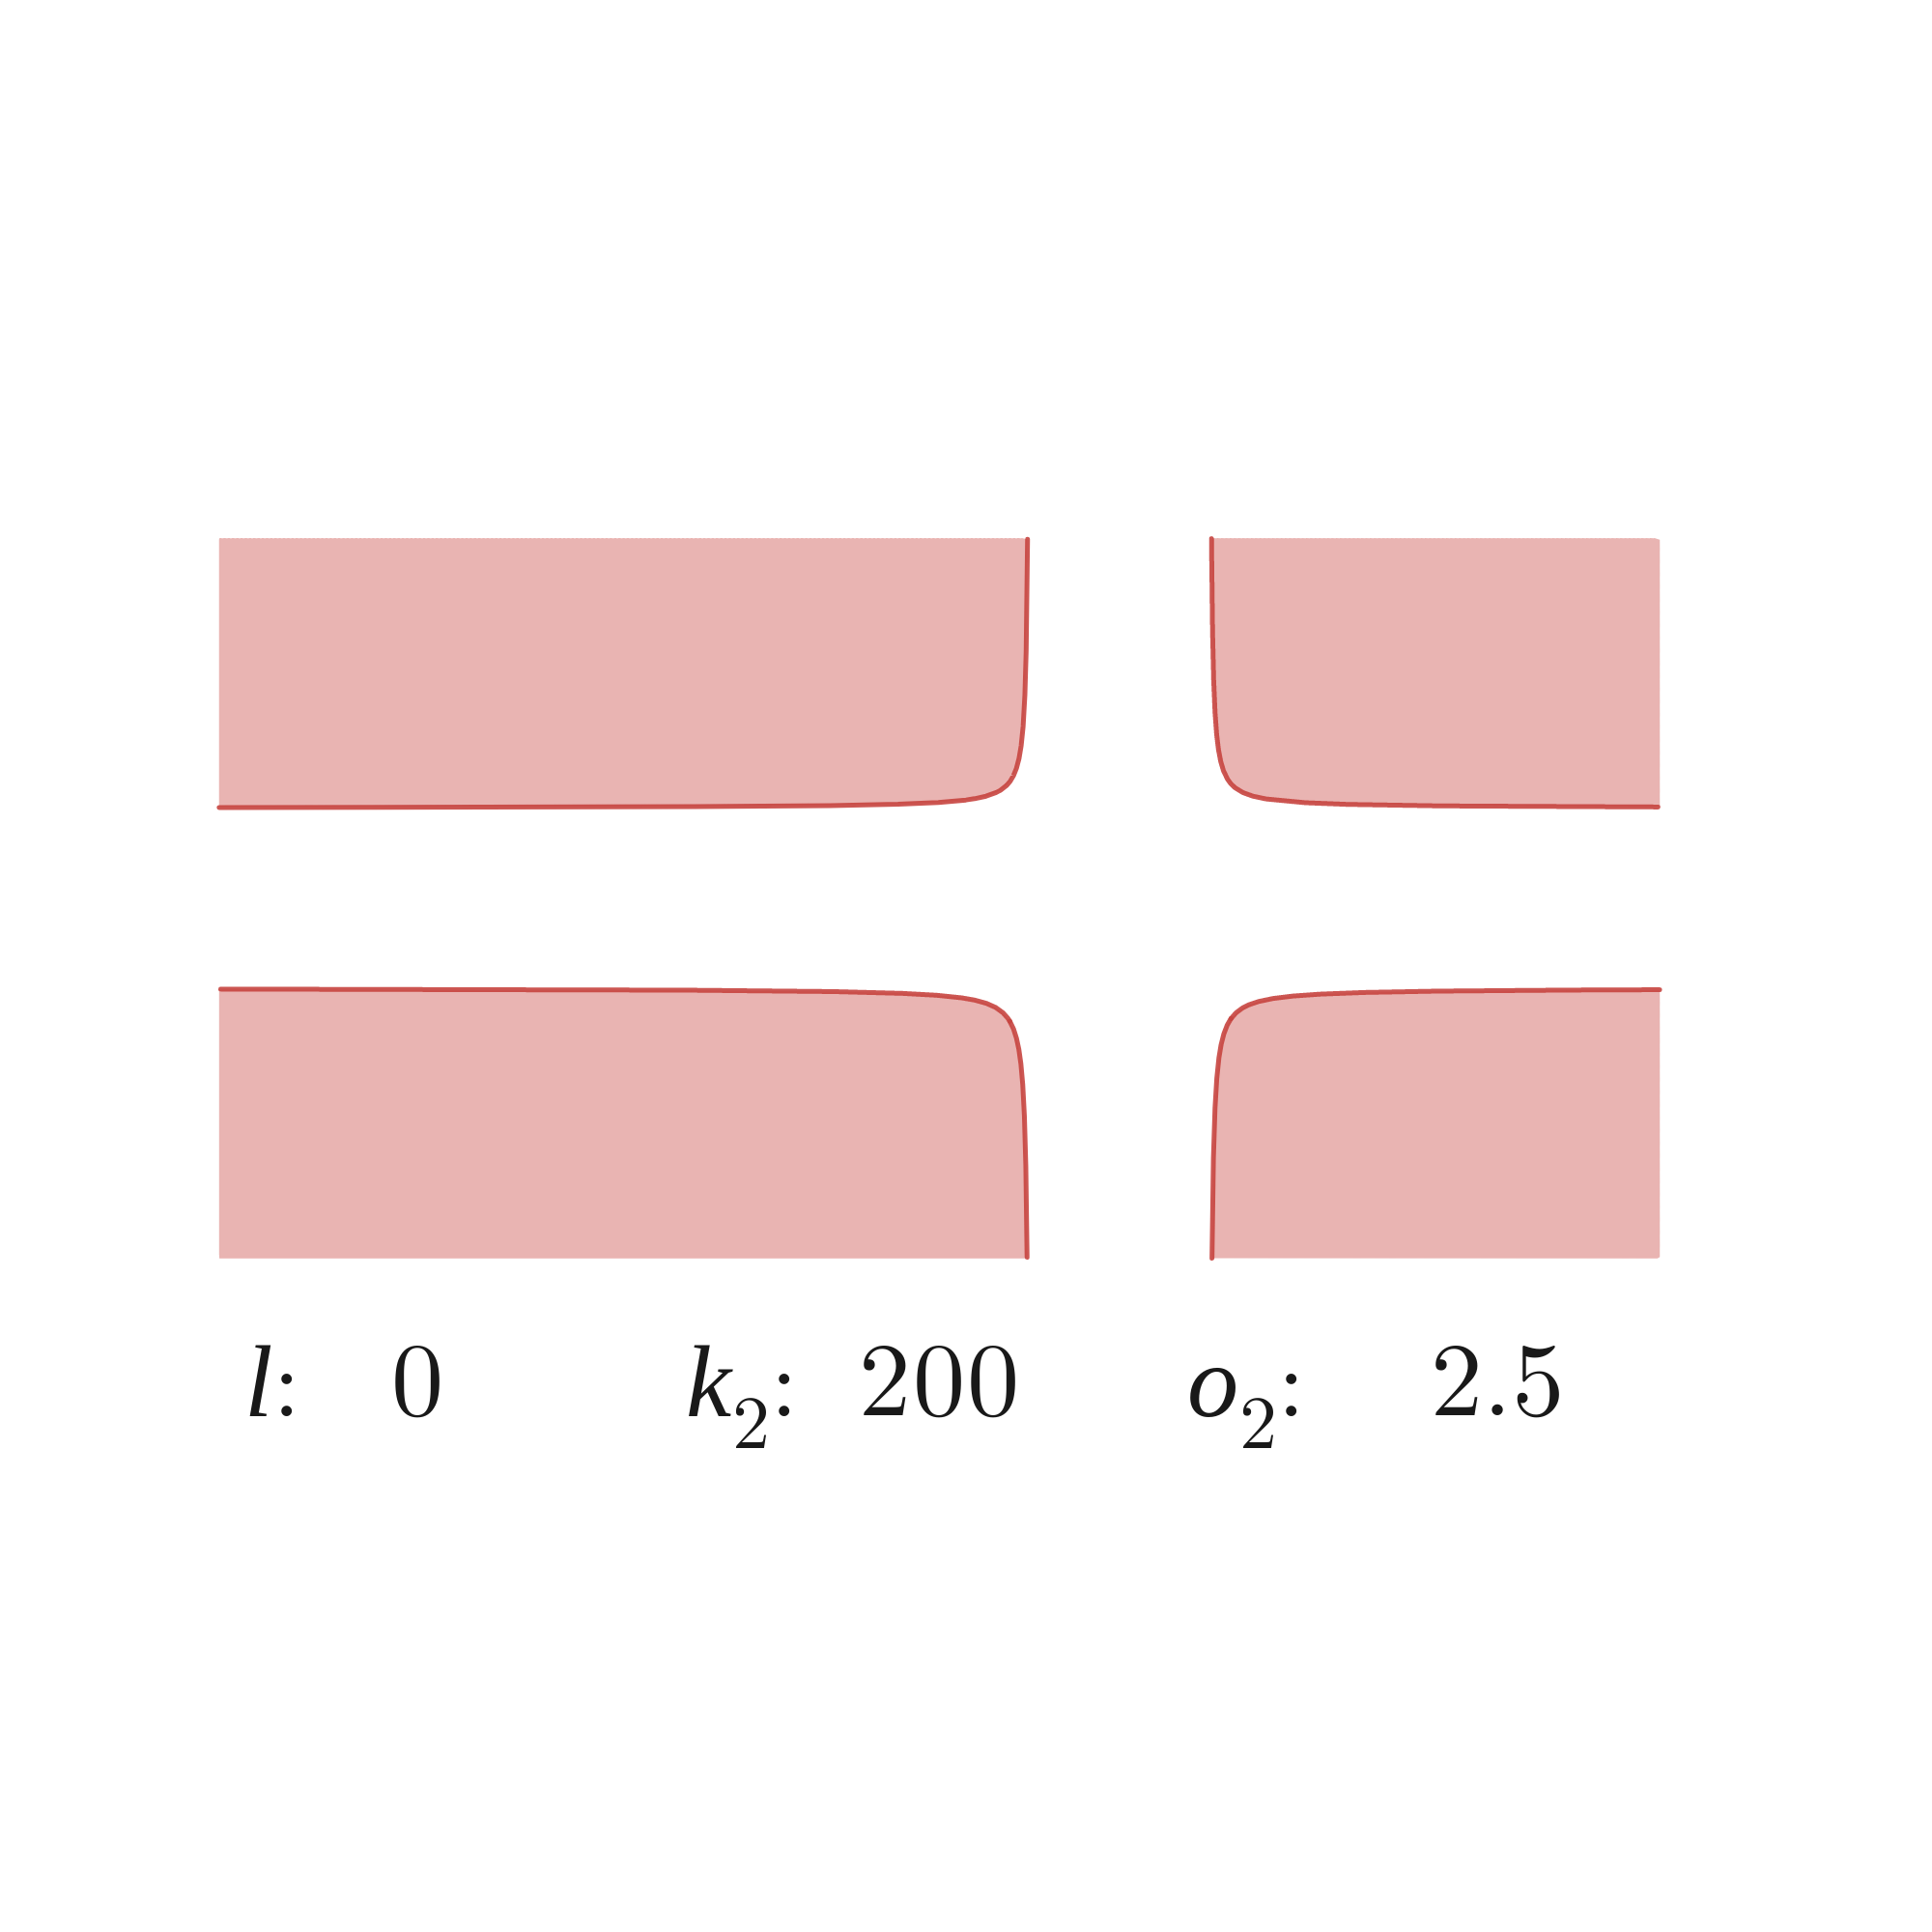
\includegraphics[width=1.\linewidth, trim={5cm 6cm 8cm 19cm}, clip]{Images/a.png}		
			\end{figure}
		\end{column}
		\begin{column}{.42\textwidth}
			\vspace{-15mm}
			\begin{figure}
				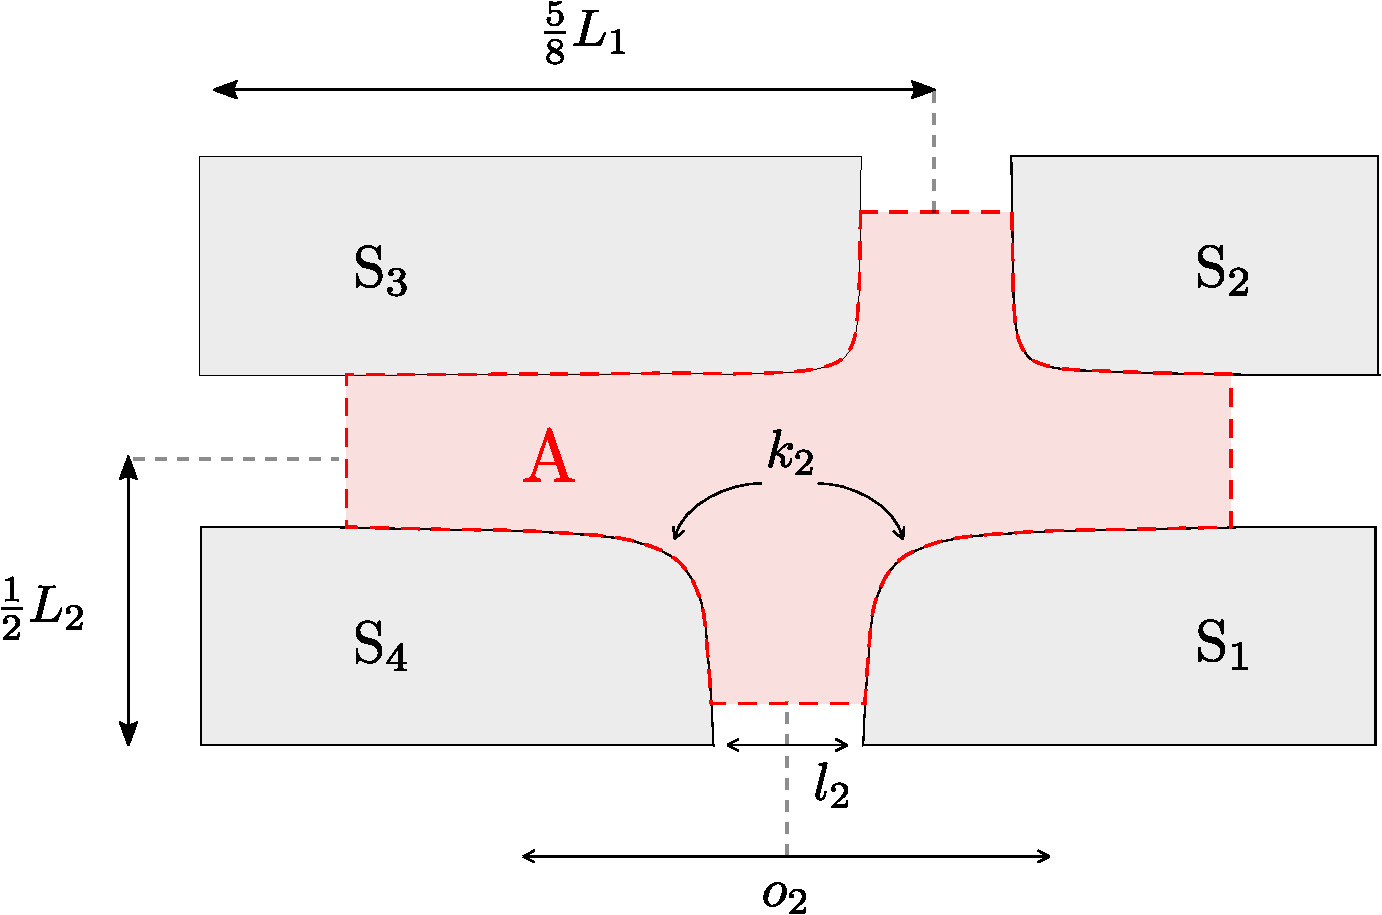
\includegraphics[width=1.\linewidth, trim={0 0 0 0}, clip]{Images/krizovatka.pdf}		
			\end{figure}
			\vspace{-3mm}
			\begin{subequations}\label{eq:tcpc vazby}
				\begin{eqnarray}
				1{,}25 &\leq& o_2 \hspace{1.5mm}\leq  \hspace{1.5mm}2{,}75 \, \nonumber,\\[3pt]
				-0{,}05 &\leq& l_2 \hspace{2.5mm}\leq \hspace{1.5mm}0{,}05 \, \nonumber,\\[3pt]
				50 &\leq& k_2 \hspace{2mm}\leq \hspace{1.5mm}200 \, \nonumber.
				\end{eqnarray}
			\end{subequations}
		\end{column}
	\end{columns}
\end{frame}
%------------------------------------------------
\begin{frame}{3 parameters - simplified TCPC model}
	\begin{itemize}
		\item 3 optimization parameters
	\end{itemize}
	\begin{columns}
		\begin{column}{.58\textwidth}
			\begin{figure}
				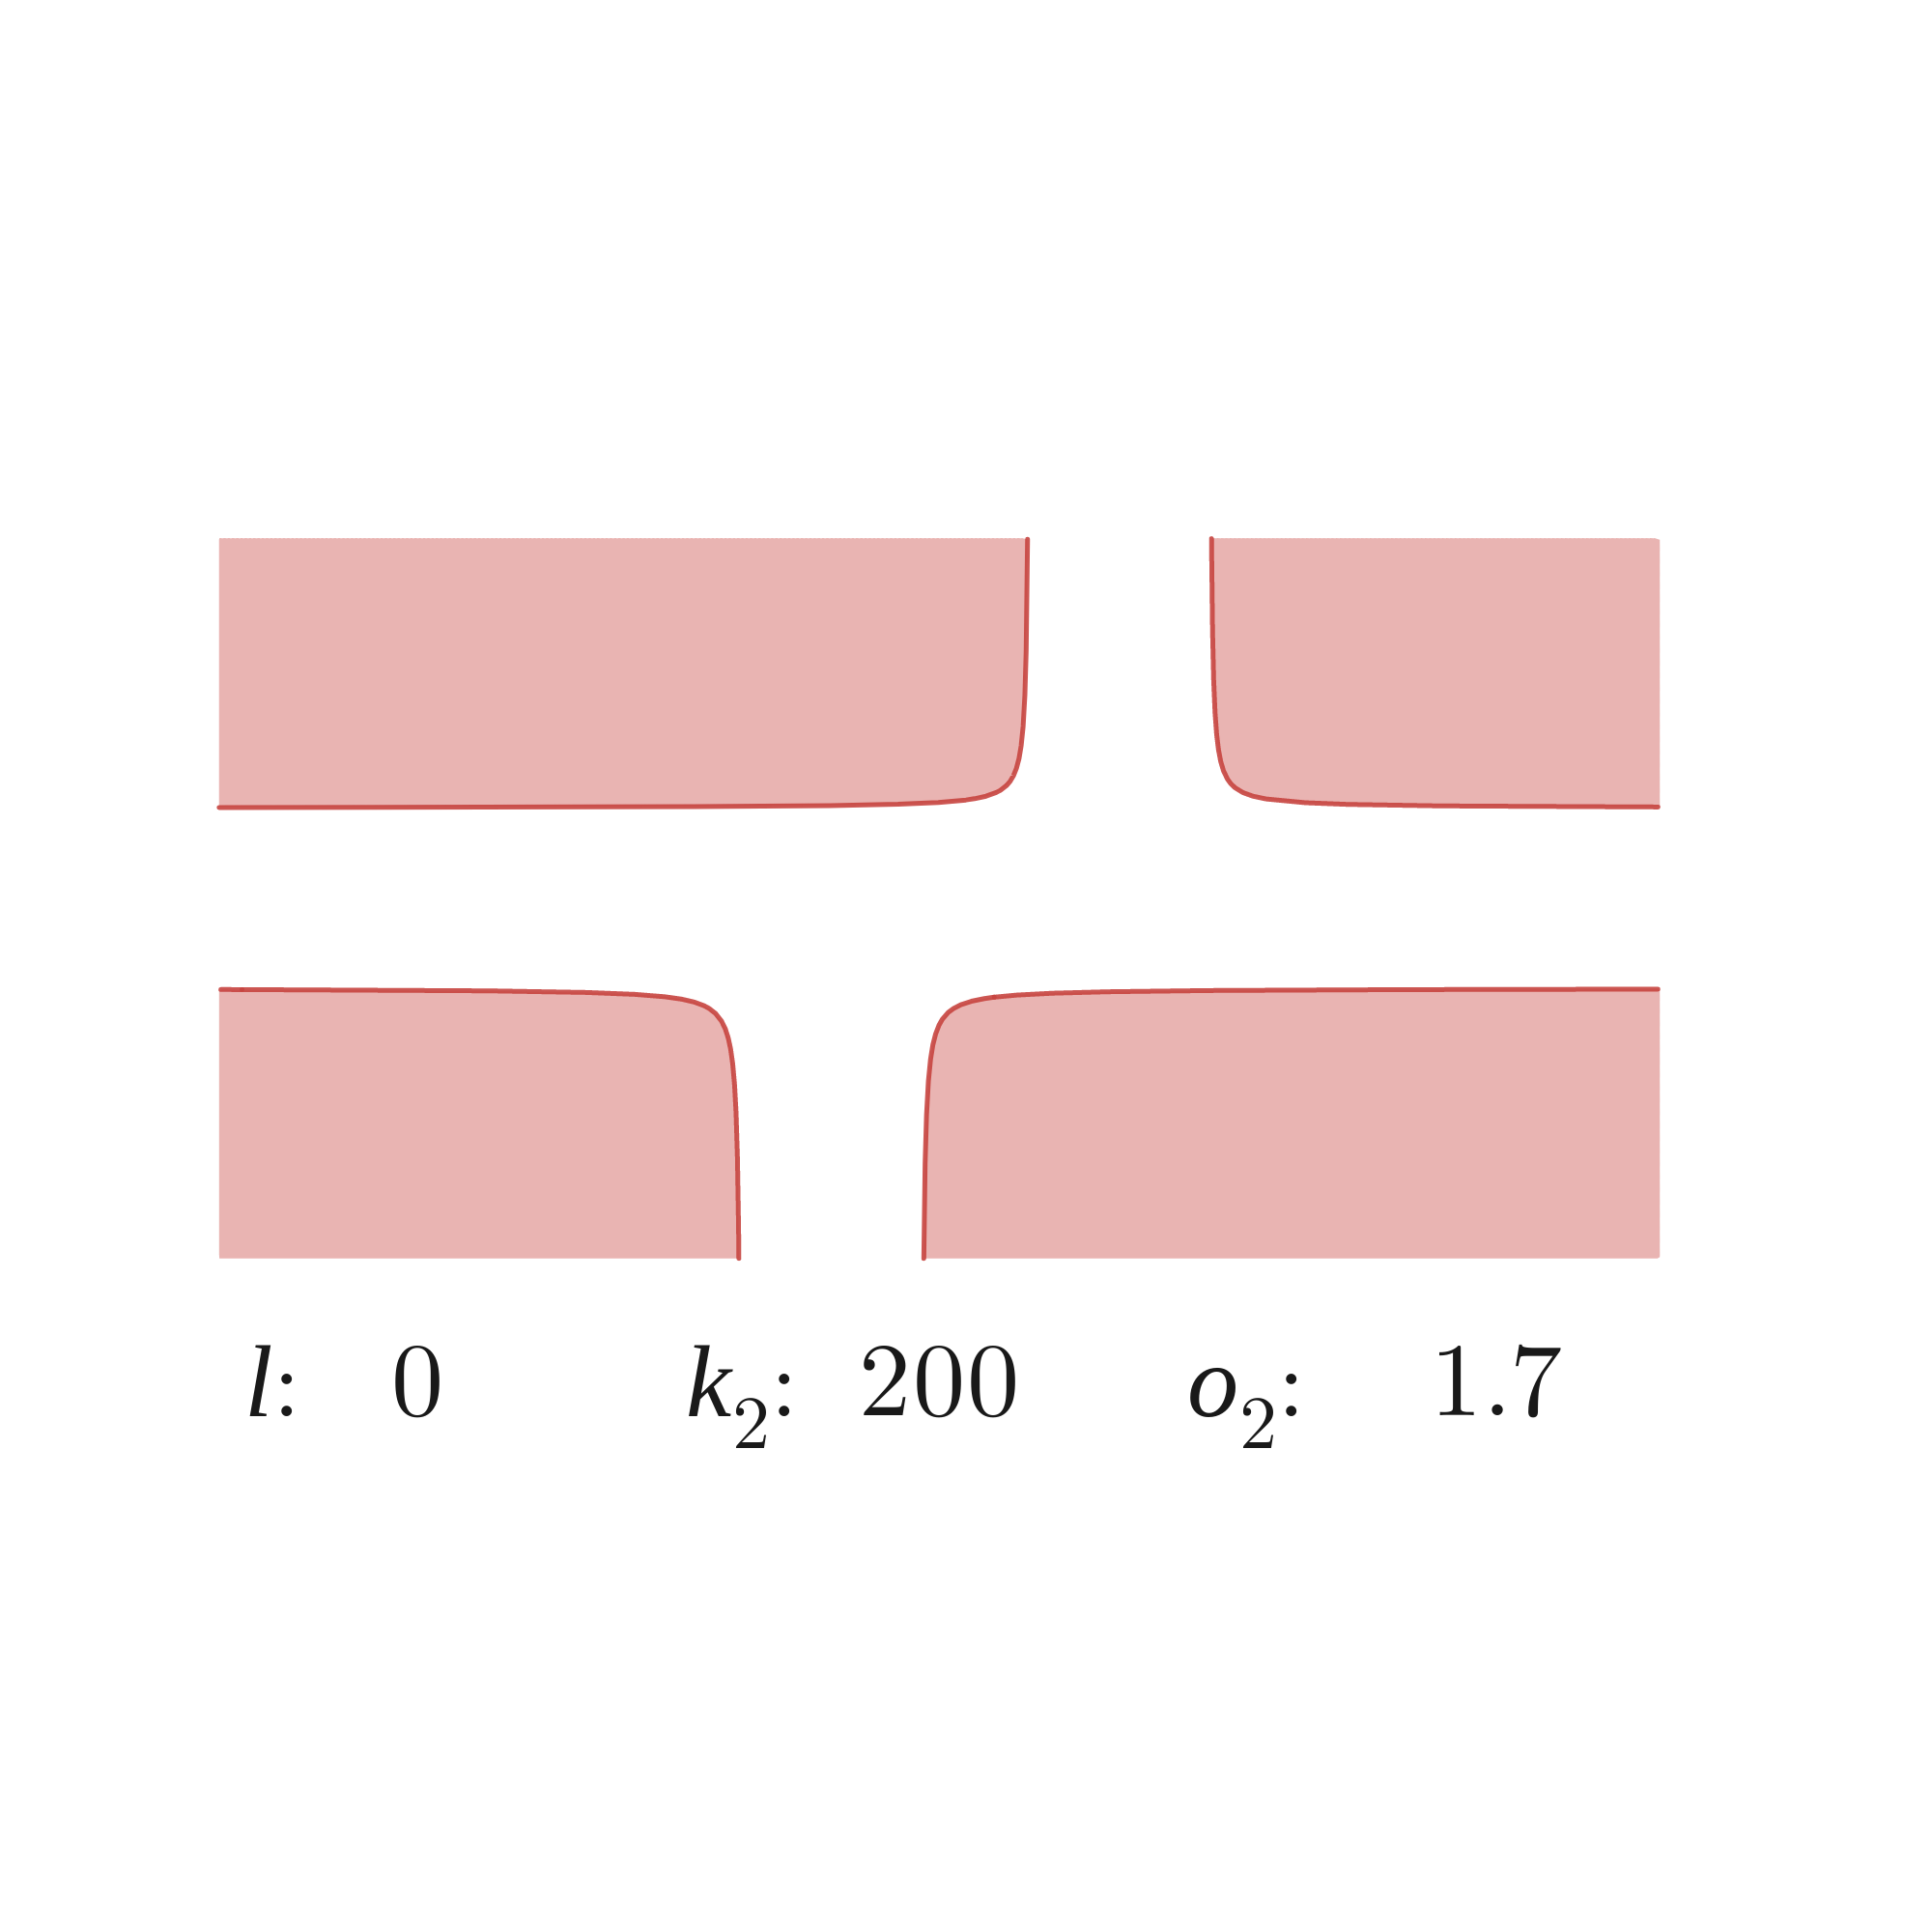
\includegraphics[width=1.\linewidth, trim={5cm 6cm 8cm 19cm}, clip]{Images/b.png}		
			\end{figure}
		\end{column}
		\begin{column}{.42\textwidth}
			\vspace{-15mm}
			\begin{figure}
				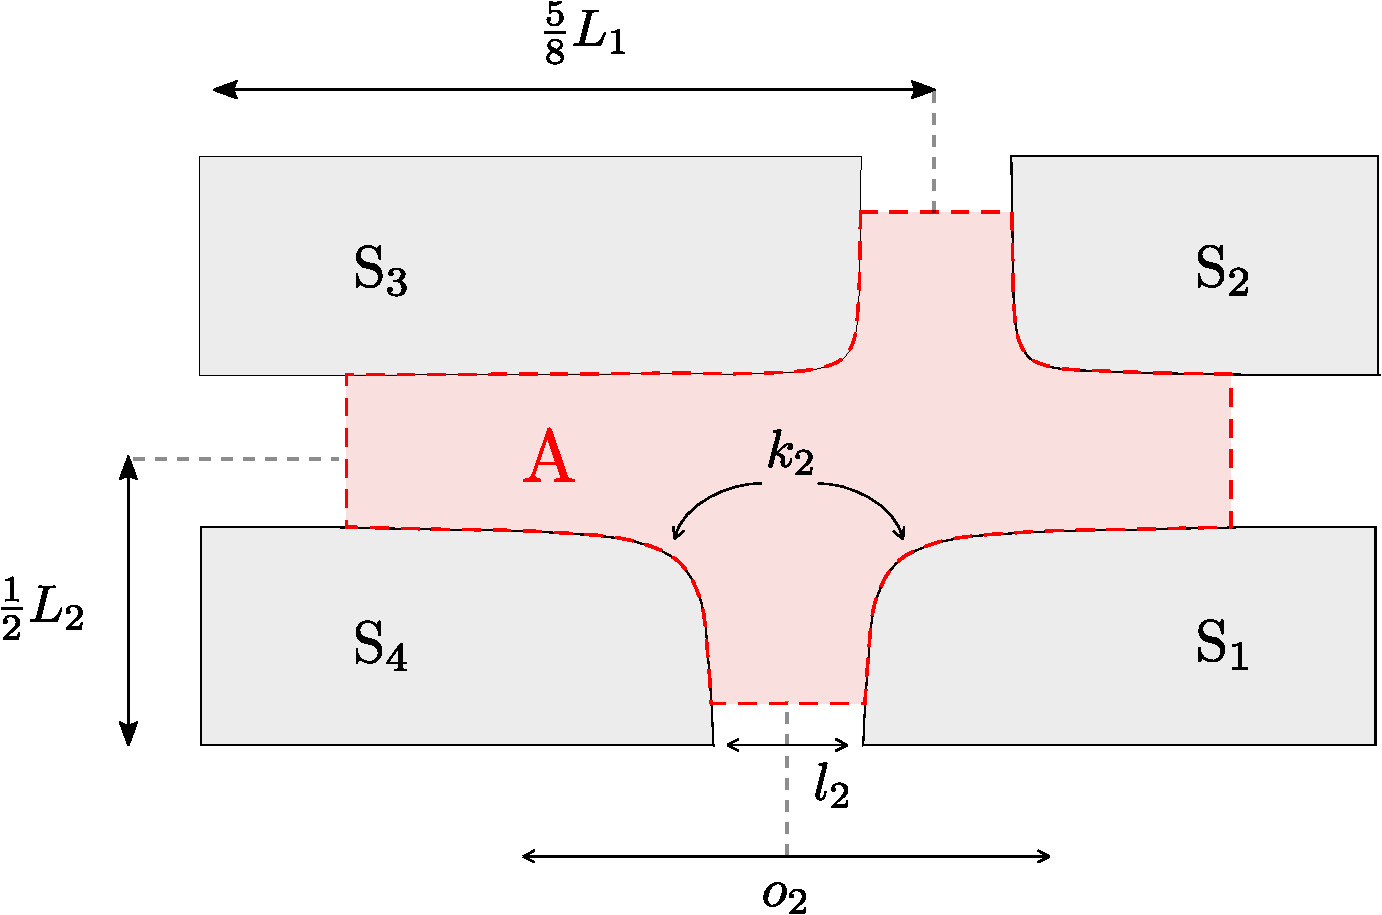
\includegraphics[width=1.\linewidth, trim={0 0 0 0}, clip]{Images/krizovatka.pdf}		
			\end{figure}
			\vspace{-3mm}
			\begin{subequations}\label{eq:tcpc vazby}
				\begin{eqnarray}
				1{,}25 &\leq& o_2 \hspace{1.5mm}\leq  \hspace{1.5mm}2{,}75 \, \nonumber,\\[3pt]
				-0{,}05 &\leq& l_2 \hspace{2.5mm}\leq \hspace{1.5mm}0{,}05 \, \nonumber,\\[3pt]
				50 &\leq& k_2 \hspace{2mm}\leq \hspace{1.5mm}200 \, \nonumber.
				\end{eqnarray}
			\end{subequations}
		\end{column}
	\end{columns}
\end{frame}
%------------------------------------------------
\begin{frame}{3 parameters - simplified TCPC model}
	\begin{itemize}
		\item 3 optimization parameters
	\end{itemize}
	\begin{columns}
		\begin{column}{.58\textwidth}
			\begin{figure}
				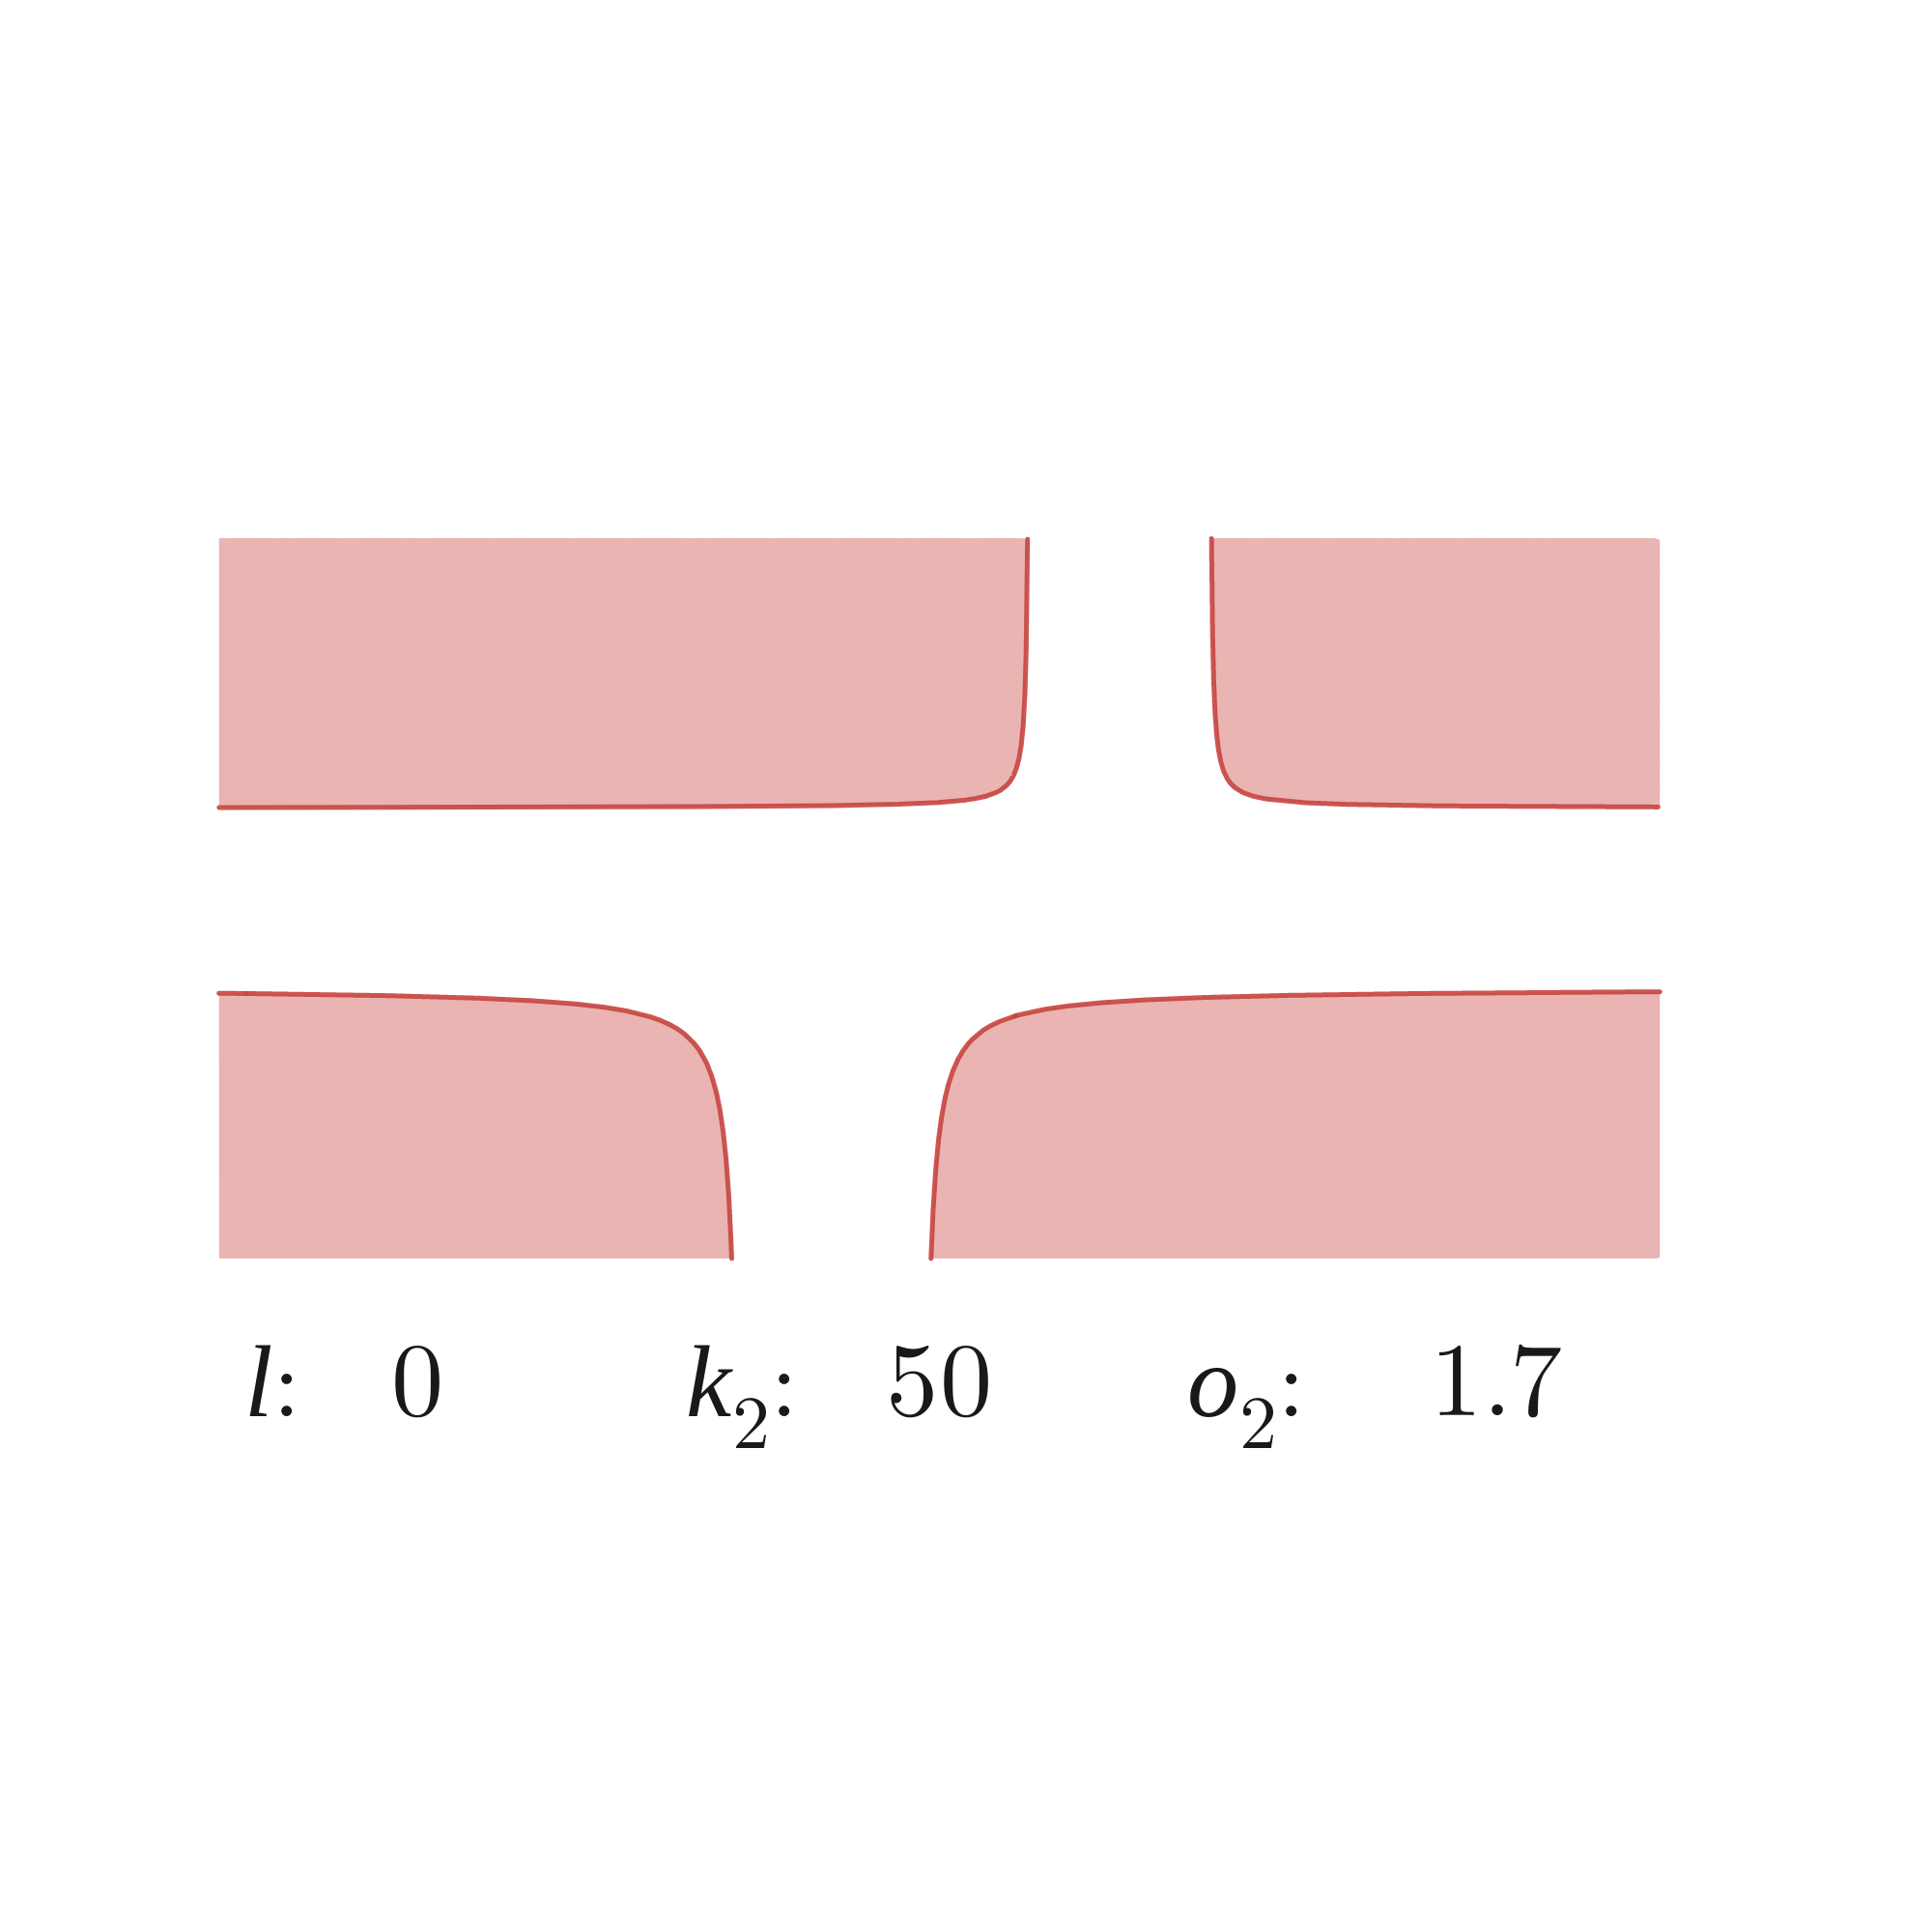
\includegraphics[width=1.\linewidth, trim={5cm 6cm 8cm 19cm}, clip]{Images/c.png}		
			\end{figure}
		\end{column}
		\begin{column}{.42\textwidth}
			\vspace{-15mm}
			\begin{figure}
				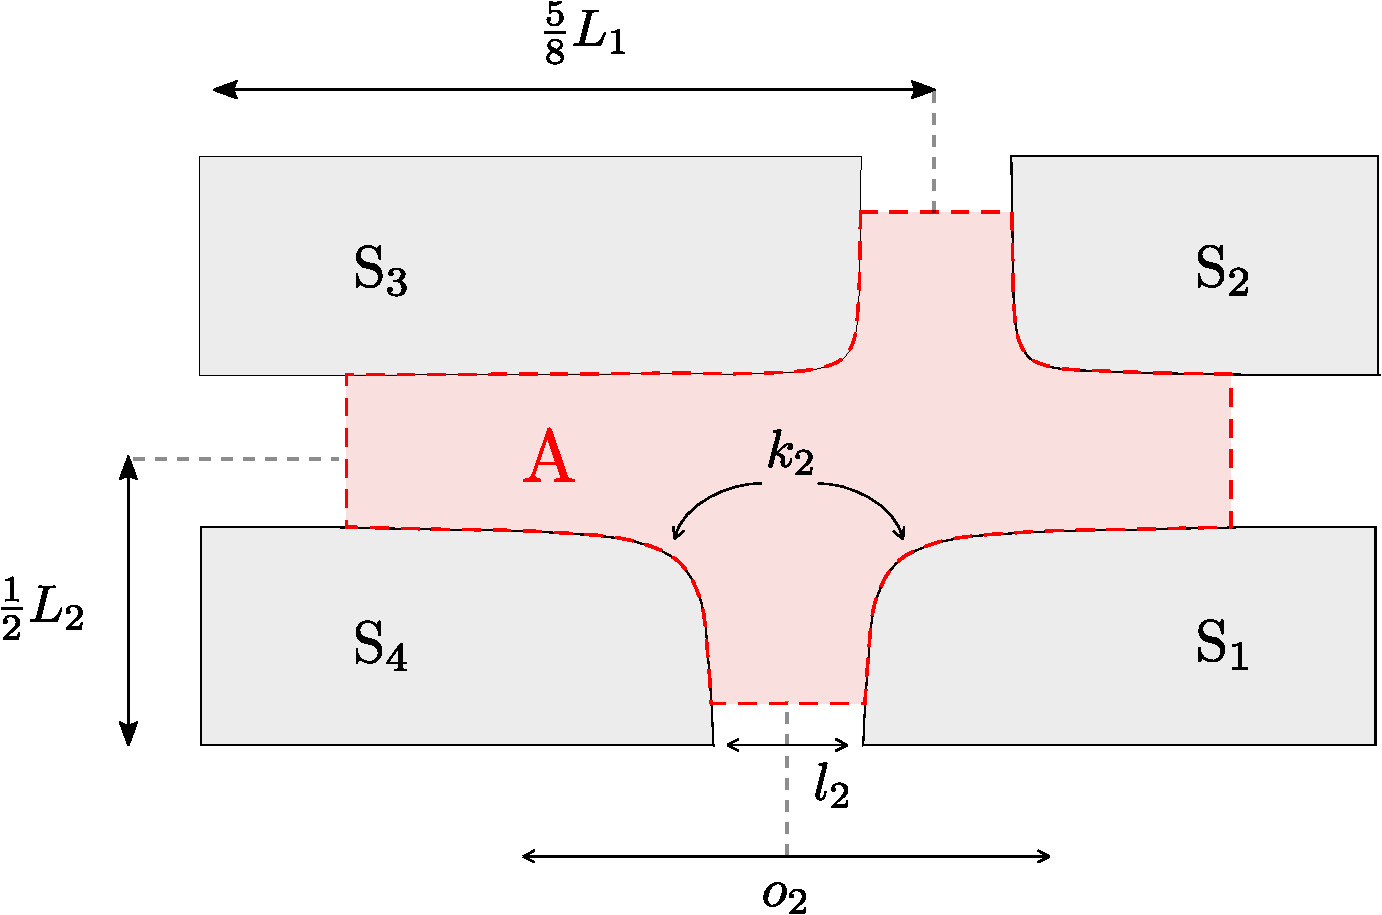
\includegraphics[width=1.\linewidth, trim={0 0 0 0}, clip]{Images/krizovatka.pdf}		
			\end{figure}
			\vspace{-3mm}
			\begin{subequations}\label{eq:tcpc vazby}
				\begin{eqnarray}
				1{,}25 &\leq& o_2 \hspace{1.5mm}\leq  \hspace{1.5mm}2{,}75 \, \nonumber,\\[3pt]
				-0{,}05 &\leq& l_2 \hspace{2.5mm}\leq \hspace{1.5mm}0{,}05 \, \nonumber,\\[3pt]
				50 &\leq& k_2 \hspace{2mm}\leq \hspace{1.5mm}200 \, \nonumber.
				\end{eqnarray}
			\end{subequations}
		\end{column}
	\end{columns}
\end{frame}
%------------------------------------------------
\begin{frame}{3 parameters - simplified TCPC model}
	\begin{itemize}
		\item 3 optimization parameters
	\end{itemize}
	\begin{columns}
		\begin{column}{.58\textwidth}
			\begin{figure}
				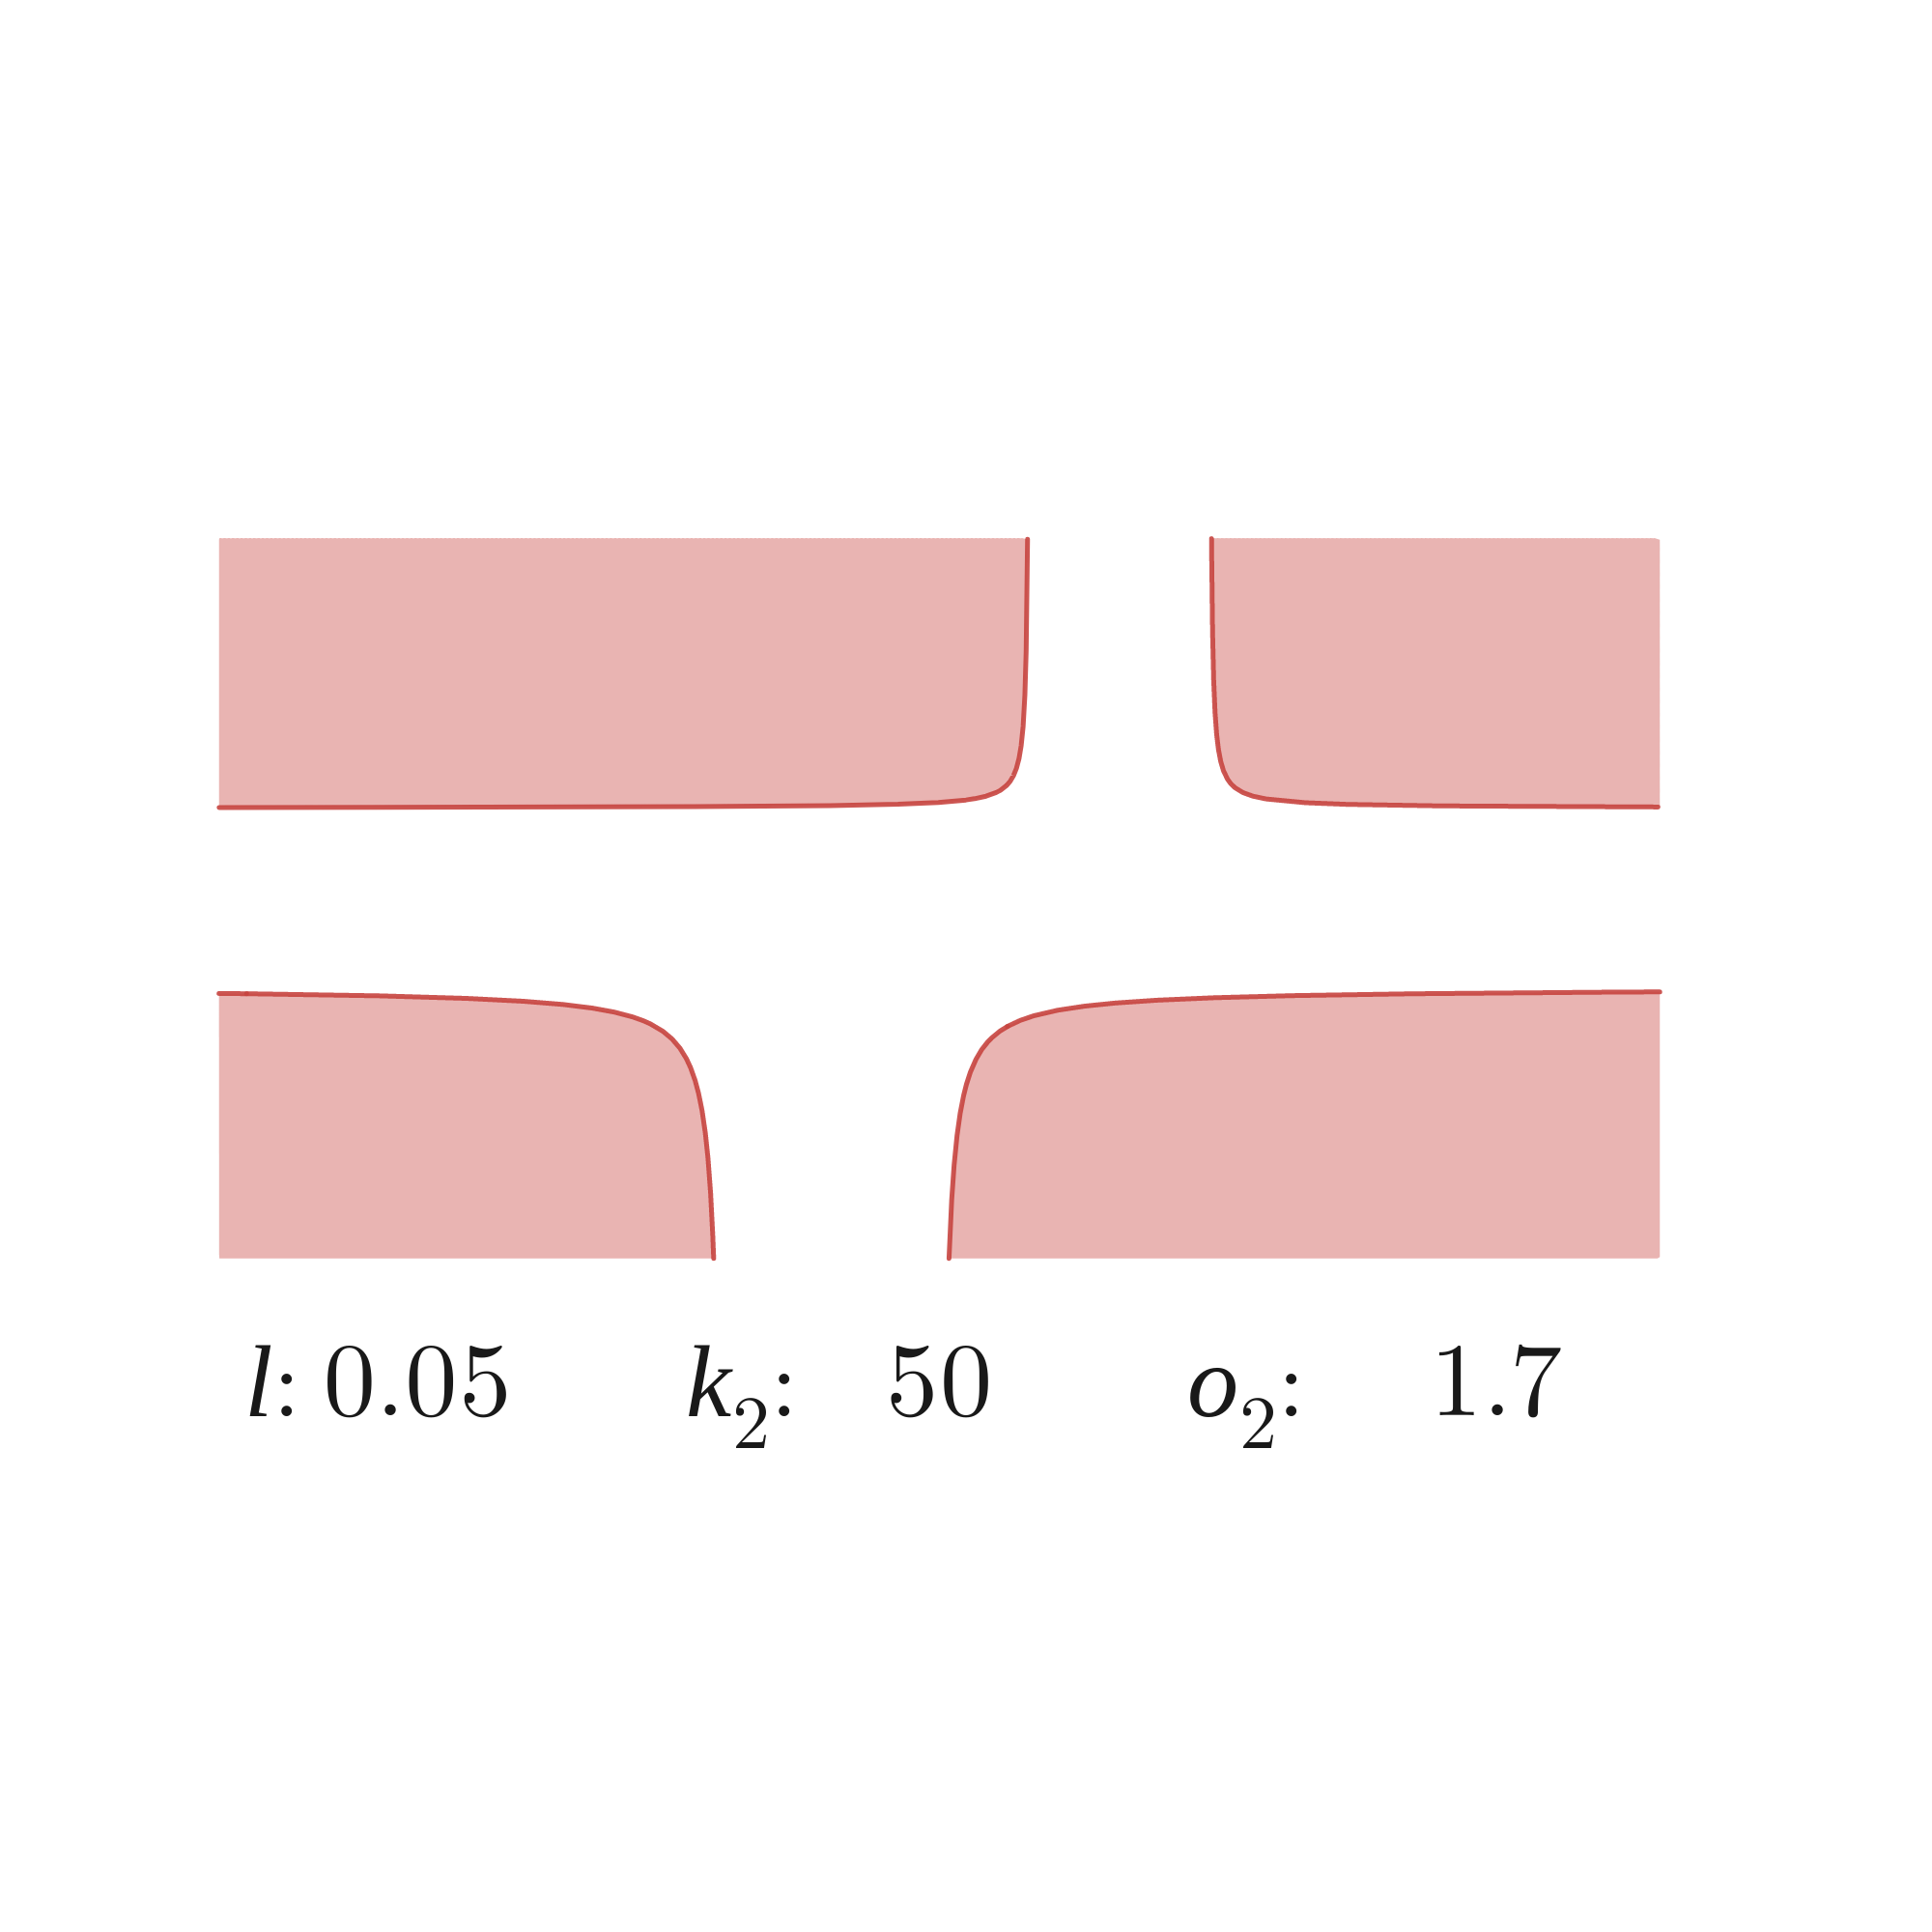
\includegraphics[width=1.\linewidth, trim={5cm 6cm 8cm 19cm}, clip]{Images/d.png}		
			\end{figure}
		\end{column}
		\begin{column}{.42\textwidth}
			\vspace{-15mm}
			\begin{figure}
				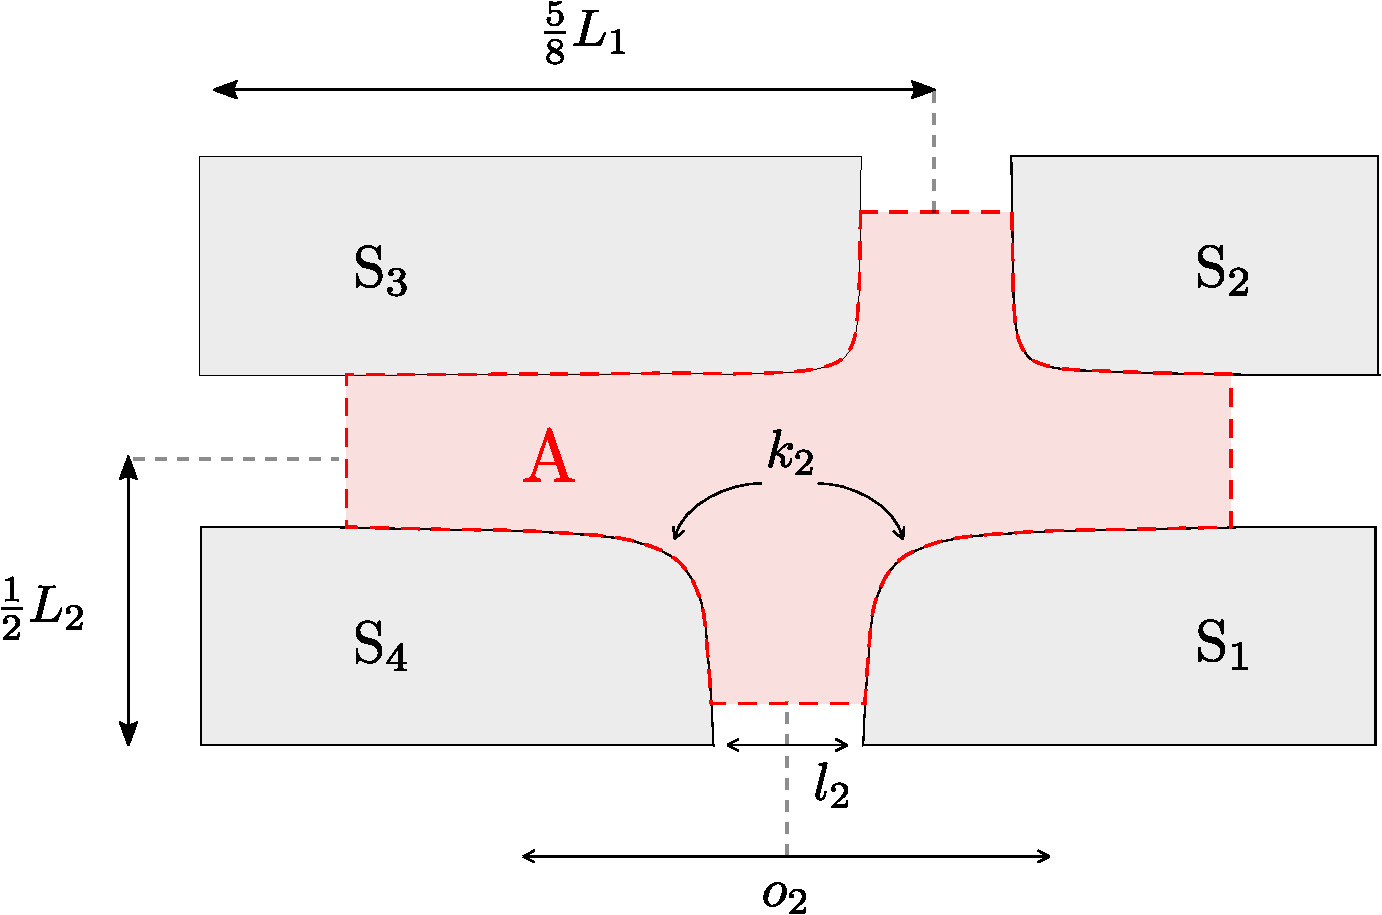
\includegraphics[width=1.\linewidth, trim={0 0 0 0}, clip]{Images/krizovatka.pdf}		
			\end{figure}
			\vspace{-3mm}
			\begin{subequations}\label{eq:tcpc vazby}
				\begin{eqnarray}
				1{,}25 &\leq& o_2 \hspace{1.5mm}\leq  \hspace{1.5mm}2{,}75 \, \nonumber,\\[3pt]
				-0{,}05 &\leq& l_2 \hspace{2.5mm}\leq \hspace{1.5mm}0{,}05 \, \nonumber,\\[3pt]
				50 &\leq& k_2 \hspace{2mm}\leq \hspace{1.5mm}200 \, \nonumber.
				\end{eqnarray}
			\end{subequations}
		\end{column}
	\end{columns}
\end{frame}
%------------------------------------------------
\begin{frame}{Minimizing the shear rate}
	$ l = -0{,}004, k_2 = 161, o_2 = 2{,}33$
	\begin{figure}[H]
		\centering
		\vspace{3mm}
		\includegraphics[width=0.75\textwidth]
		%		{Images/tcpc/tcpc_dotgamma_veloc_a.png}\\[10pt]
		{Images/tcpc_dotgamma_veloc_a_streamlines.png}\\[11pt]
		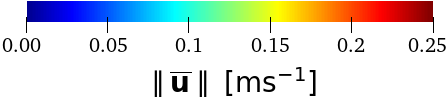
\includegraphics[width=0.37	\textwidth]{Images/tcpc_dotgamma_veloc_legenda.png}
	\end{figure}
\end{frame}
%------------------------------------------------
\begin{frame}{Minimizing the shear rate}
	\addtocounter{framenumber}{-1}
	\begin{columns}
		\begin{column}{.65\textwidth}
			\begin{figure}
				\vspace{2mm}
				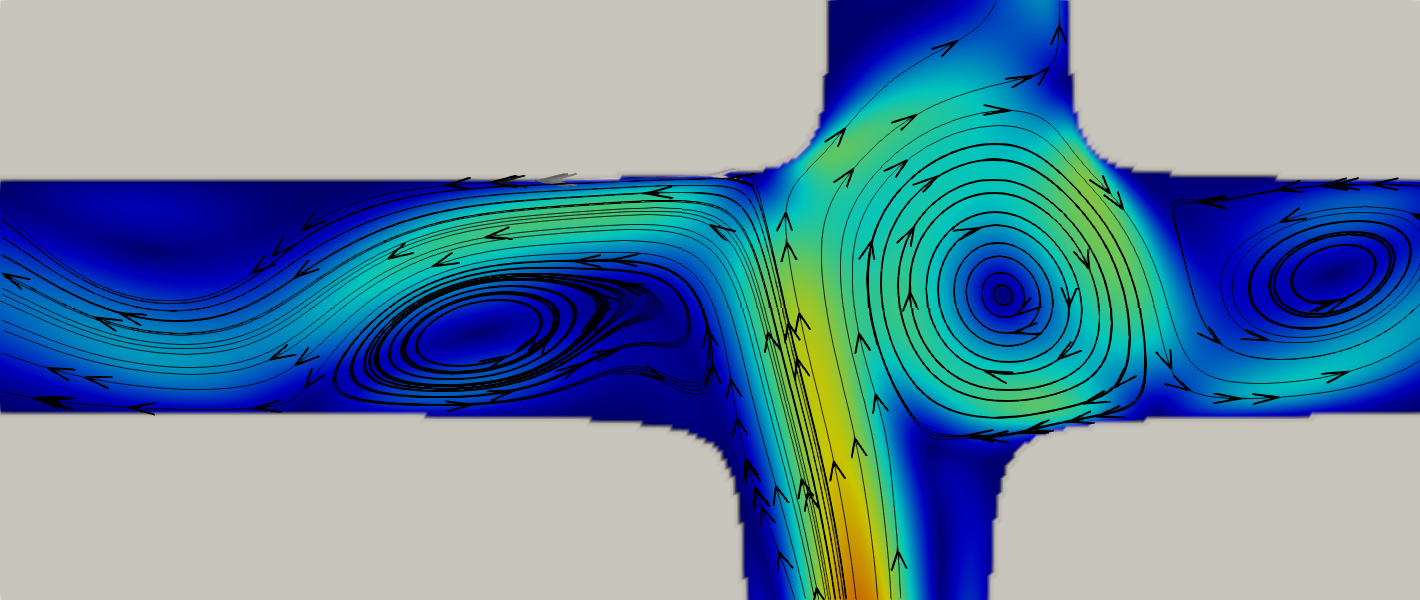
\includegraphics[width=1.0\linewidth, trim={0 0 1cm 9mm}, clip]{Images/tcpc_dotgamma_veloc_a_streamlines.png}
				\\[7pt]
				\includegraphics[width=0.37	\textwidth]{Images/tcpc_dotgamma_veloc_legenda.png}
			\end{figure}
		\end{column}
		\begin{column}{.35\textwidth}
			%			\hspace{1mm}Nelder-Mead:
			\begin{figure}
				\renewcommand{\figurename}{Fontan circulation}
				\includegraphics[width=0.75\linewidth, trim={0 0 0 0mm}, clip]{Images/vortex.png}
				\caption{[3]}		
			\end{figure}
			%			\vspace{0.8cm}
			%			\hspace{1mm}L-BFGS:
			%			\begin{figure}
			%				\includegraphics[width=1.0\linewidth, trim={0 0 0 9mm}, clip]{Images/bfgs.png}		
			%			\end{figure}
		\end{column}
	\end{columns}	
	\vspace{-1mm}
	\tiny{[3] Rijnberg F. (2018), \textit{Energetics of Blood Flow in Cardiovascular
			Disease
		}, doi: 10.1161/CIRCULATIONAHA.117.033359}
\end{frame}
%------------------------------------------------
\begin{frame}{Minimizing the turbulence kinetic energy}
	$ l = 0{,}002, k_2 = 167, o_2 = 2{,}75$
	\begin{figure}[H]
		\centering
		\vspace{3mm}
		\includegraphics[width=0.75
		\textwidth]{Images/tcpc_tke_veloc_a3.png}\\[11pt]
		\includegraphics[width=0.37	\textwidth]{Images/tcpc_dotgamma_veloc_legenda.png}
	\end{figure}
\end{frame}
%------------------------------------------------
\begin{frame}{Comparison of $ \dot{\gamma} $}
	\addtocounter{framenumber}{-1}
	\begin{columns}
		\begin{column}{.42\textwidth}
			\begin{figure}
				\vspace{-1mm}
				Min shear rate:
				\includegraphics[width=0.8\linewidth, trim={0 0 0cm 0mm}, clip]{Images/gamma_frame.pdf}		
			\end{figure}
		\end{column}
		\begin{column}{.42\textwidth}
			%			\hspace{1mm}Nelder-Mead:
			\begin{figure}
				\vspace{-1mm}
				Min turbulent kinetic energy:
				\includegraphics[width=0.8\linewidth, trim={0 0 0 0mm}, clip]{Images/tke_frame.pdf}		
			\end{figure}
		\end{column}
	\end{columns}
	\centering
	\vspace{3mm}
	\includegraphics[width=0.35	\textwidth, trim={0 0 0mm 0mm}, clip]{Images/tcpc_dotgamma_dotgamma_ legenda.png}
\end{frame}

%------------------------------------------------

\begin{frame}{Summary}
	\begin{itemize}
		\setlength\itemsep{1.4em}
		\item Framework to generate and solve optimization problems using LBM
		\item Answering non-trivial questions
		\item Plans: 3D, TCP connection, finding sufficient objective function
	\end{itemize}\pause
	\vspace{9mm}
	\huge{\centerline{\textbf{Thank you for your attention!}}}
\end{frame}
%------------------------------------------------
%\begin{frame}{References}
%    % Beamer does not support BibTeX so references must be inserted manually as below
%    \footnotesize{
%    	\begin{thebibliography}{99}
%    		\bibitem[Smith, 2012]{p1} [1] Eichler P., Fučík R., Strachota P. (2022)
%    		\newblock Investigation of mesoscopic boundary conditions for lattice Boltzmann method
%    		in laminar flow problems.
%    		\newblock preprint submitted to \emph{Comput. Math. with Appl.}.
%    	\end{thebibliography}
%    }
%    \footnotesize{
%        \begin{thebibliography}{99}
%            \bibitem[Smith, 2012]{p1} [2] Bouzidi M., Firdaouss M., Lallemand P. (2001)
%            \newblock Momentum transfer of a Boltzmann-lattice fluid with boundaries.
%            \newblock \emph{Physics of Fluids} 13(11), 3452–3459.
%        \end{thebibliography}
%    }
%    \footnotesize{
%	\begin{thebibliography}{99}
%		\bibitem[Smith, 2012]{p1} [3] Rijnberg F.~M., et al. (2018)
%		\newblock {E}nergetics of blood flow in cardiovascular disease.
%		\newblock \emph{Circulation} 137(22):2393--2407,2018.
%	\end{thebibliography}
%	}
%	\vspace{0.7cm}
%
%	All uncited figures are either original or in public domain.
%
%\end{frame}

%------------------------------------------------
%
%\begin{frame}
%    \Huge{\centerline{\textbf{Thank you for your attention!}}}
%\end{frame}

%----------------------------------------------------------------------------------------
\end{document}